\documentclass[12pt,a4paper,twoside]{report}
% -------------------------------------------------------------------- %
% Pacotes

\usepackage[utf8]{inputenc}
\usepackage[T1]{fontenc}
\usepackage[brazil]{babel}
\usepackage[fixlanguage]{babelbib}
\usepackage[pdftex]{graphicx}      % usamos arquivos pdf/png como figuras
\usepackage{setspace}              % espaçamento flexvel
\usepackage{indentfirst}           % indentação do primeiro parágrafo
\usepackage{makeidx}               % índice remissivo
\usepackage[nottoc]{tocbibind}     % acrescentamos a bibliografia/indice/conteudo no Table of Contents
\usepackage{courier}               % usa o Adobe Courier no lugar de Computer Modern Typewriter
\usepackage{type1cm}               % fontes realmente escaláveis
\usepackage{titletoc}
\usepackage{ucs}
\usepackage[font=small,format=plain,labelfont=bf,up,textfont=it,up]{caption}
\usepackage[usenames,svgnames,dvipsnames]{xcolor}
\usepackage[a4paper,top=2.54cm,bottom=2.0cm,left=2.0cm,right=2.54cm]{geometry} % margens
\usepackage{amsmath} 
\usepackage{float}

\usepackage[pdftex,plainpages=false,pdfpagelabels,pagebackref,colorlinks=true,citecolor=DarkGreen,
linkcolor=NavyBlue,urlcolor=DarkRed,filecolor=green,bookmarksopen=true]{hyperref} % links coloridos
\usepackage[all]{hypcap}                % soluciona o problema com o hyperref e capítulos
\usepackage[square,sort,nonamebreak,comma]{natbib}  % citação bibliográfica alpha
\fontsize{60}{62}\usefont{OT1}{cmr}{m}{n}{\selectfont}
\usepackage{upquote}                    % formata apóstrofes '
\usepackage{textcomp}

% Para formatar corretamente as URLs
\usepackage{url}
% -------------------------------------------------------------------- %
% Cabeçalhos similares ao TAOCP de Donald E. Knuth
\usepackage{fancyhdr}
\pagestyle{fancy}
\fancyhf{}
\renewcommand{\chaptermark}[1]{\markboth{\MakeUppercase{#1}}{}}
\renewcommand{\sectionmark}[1]{\markright{\MakeUppercase{#1}}{}}
\renewcommand{\headrulewidth}{0pt}

% -------------------------------------------------------------------- %
\graphicspath{{./imagens/}}        % caminho das figuras
\frenchspacing                     % arruma o espaço: id est (i.e.) e exempli gratia (e.g.)
\urlstyle{same}                    % URL com o mesmo estilo do texto e no mono-spaced
\makeindex                         % para o índice remissivo
\raggedbottom                      % para no permitir espaços extras no texto
\fontsize{60}{62}\usefont{OT1}{cmr}{m}{n}{\selectfont}
\cleardoublepage
\normalsize

% -------------------------------------------------------------------- %
% Cores para formatação de código
\usepackage{color}
\definecolor{vermelho}{rgb}{0.6,0,0} % para strings
\definecolor{verde}{rgb}{0.25,0.5,0.35} % para comentários
\definecolor{roxo}{rgb}{0.5,0,0.35} % para palavras-chaves
\definecolor{azul}{rgb}{0.25,0.35,0.75} % para strings
\definecolor{cinza-claro}{gray}{0.95}
% -------------------------------------------------------------------- %
% Opções de listagem usados para o código fonte
% Ref: http://en.wikibooks.org/wiki/LaTeX/Packages/Listings



\usepackage{listings}           % para formatar código-fonte (ex. em Java)


\lstset{ %
language=[Objective]Caml,  % seleciona a linguagem do código (aqui em lstlang0.sty
basicstyle=\footnotesize\ttfamily, % o tamanho da fonte usado no código
commentstyle=\color{verde}\bfseries,  % formatação de comentários
stringstyle=\color{azul},    % formatação de strings
upquote=true,
numbers=left,                   % onde colocar os números de linha
numberstyle=\tiny,  % o tamanho da fonte usada para a numeração das linhas
stepnumber=1,                   % o intervalo entre dois números de linhas. Se for 1, numera cada uma.
numbersep=5pt,                  % how far the line-numbers are from the code
showspaces=false,               % show spaces adding particular underscores
showstringspaces=false,         % underline spaces within strings
showtabs=false,                 % show tabs within strings adding particular underscores
keywordstyle=\color{roxo}\bfseries,
keywordstyle=[1]\color{roxo}\bfseries,
keywordstyle=[2]\color{verde}\bfseries,
%        keywordstyle=[3]\textbf,    %
%        keywordstyle=[4]\textbf,   \sqrt{\sqrt{}} %
frame=b,                   % adds a frame around the code
framerule=0.6pt,
tabsize=2,                      % sets default tabsize to 2 spaces
captionpos=t,                   % sets the caption-position to top
breaklines=true,                % sets automatic line breaking
breakatwhitespace=false,        % sets if automatic breaks should only happen at whitespace
escapeinside={\%*}{*)},         % if you want to add a comment within your code
backgroundcolor=\color[rgb]{1.0,1.0,1.0}, % choose the background color.
rulecolor=\color[rgb]{0.8,0.8,0.8},
extendedchars=true,
xleftmargin=10pt,
xrightmargin=10pt,
framexleftmargin=10pt,
framexrightmargin=10pt,
literate={â}{{\^{a}}}1  % para formatar corretamente os acentos do Português ao usar utf8
    {ê}{{\^{e}}}1
    {ô}{{\^{o}}}1  
    {Â}{{\^{A}}}1
    {Ê}{{\^{E}}}1
    {Ô}{{\^{O}}}1
    {á}{{\'{a}}}1
    {é}{{\'{e}}}1
    {í}{{\'{i}}}1
    {ó}{{\'{o}}}1
    {ú}{{\'{u}}}1
    {Á}{{\'{A}}}1
    {É}{{\'{E}}}1
    {Í}{{\'{I}}}1
    {Ó}{{\'{O}}}1
    {Ú}{{\'{U}}}1
    {à}{{\`{a}}}1
    {À}{{\`{A}}}1
    {ã}{{\~{a}}}1
    {õ}{{\~{o}}}1
    {Ã}{{\~{A}}}1
    {Õ}{{\~{O}}}1
    {ç}{{\c{c}}}1
    {Ç}{{\c{C}}}1
    {ü}{{\"u}}1
    {Ü}{{\"U}}1
}

\renewcommand{\lstlistingname}{Listagem}
\renewcommand{\lstlistlistingname}{Lista de Listagens}

% Definição de novos estilos
\lstdefinestyle{Bash}
    {language=bash,frame=single,numbers=none,basicstyle=\footnotesize\ttfamily,
     morekeywords={cp,mkdir,sudo,tar}}

% Definição de novos ambientes
\lstnewenvironment{terminal}
  {\lstset{style=Bash}}
  {}

\lstnewenvironment{ocaml}
  {\lstset{basicstyle=\scriptsize\ttfamily,
           frame=single,
           frameround=tttt,
           framerule=2pt,
           numbers=none,
           rulecolor=\color{Salmon}}}
  {}

\lstnewenvironment{xml}
   {\lstset{language=XML,frame=single,numbers=none}}
   {}

\lstnewenvironment{interprete}
  {\lstset{frame=single,
            frameround=tttt,
            numbers=none,
            basicstyle=\ttfamily,
            framerule=2pt,
            rulecolor=\color{CadetBlue}}}
  {}
% Formata o caption da listagem
% \DeclareCaptionFont{blue}{\color{blue}} 

% \captionsetup[lstlisting]{singlelinecheck=false, labelfont={blue}, textfont={blue}}
\usepackage{caption}
\DeclareCaptionFont{white}{\color{white}}
\DeclareCaptionFormat{listing}{\colorbox[cmyk]{0.43, 0.35, 0.35,0.01}{\parbox{\textwidth}{\hspace{15pt}#1#2#3}}}
\captionsetup[lstlisting]{format=listing,labelfont=white,textfont=white, singlelinecheck=false, margin=0pt, font={bf,footnotesize}}

\newcommand{\ListingsPath}{./codigos}
% Inclui o nome do arquivo como Caption 
\newcommand{\filelisting}[2][]{%
    \lstinputlisting[caption={\texttt{\detokenize{#2}}},#1]{\ListingsPath/#2}%
}

% ---------------------------------------------------------------------------- %

% ---------------------------------------------------------------------------- %

\title{Análise de Algoritmos - Ordenação}
\date{}
\author{Gustavo de Souza Silva \\ Guilherme de Souza Silva \\ Arthur Xavier \\ Schumaiquer Souto \\
\vspace{1cm} \\
Faculdade de Computação \\
Universidade Federal de Uberlândia
}
\date{\today}

%\includeonly{cap-clojure,magical,short}
\begin{document}
  \maketitle
% -------------------------------------------------------------------- %
% Listas de figuras, tabelas e códigos criadas automaticamente
\listoffigures            
\listoftables            
\lstlistoflistings
% -------------------------------------------------------------------- %

% -------------------------------------------------------------------- %
% Sumário
\tableofcontents    

% Capítulos do trabalho

% cabeçalho para as páginas de todos os capítulos
\fancyhead[RE,LO]{\thesection}

%\singlespacing              % espaçamento simples
\setlength{\parskip}{0.15in} % espaçamento entre paragráfos

\chapter{Introdução}
Este relatŕio tem como objetivo fazer a análise de diversos algoritmos já conhecidos de ordenação. O intúito desde trabalho é comprovar que as provas matemáticas realmente acontecem em um ambiente real de execução.

\section{Codificação}
O arquivo vetor.c mantém todas as funções a respeito do vetor, como geração, preenchimento, etc.
\lstinputlisting[label={arq:vetor.c}, language=C, caption={Arquivo referente ao vetor}]{../vetor.c}

Este arquivo serve para gerar os vetores e salva-los em arquivos.
\lstinputlisting[label={arq:gera_vets.c}, language=C, caption={Geração dos vetores}]{../gera_vets.c}

Este arquivo contém os algoritmos de ordenação pedidos.
\lstinputlisting[label={arq:ordena.c}, language=C, caption={Métodos de ordenação}]{../ordena.c}

O arquivo ensaios.c serve para automatizar e calcular os tempos de cada método de ordenação.
\lstinputlisting[label={arq:ensaios.c}, language=C, caption={Automatização dos experimentos}]{../ensaios.c}

\subsection{Comandos}
Os seguintes passos devem ser seguidos para criação dos vetores que serão utilizados no experimento:
1 - Compilar o arquivo vetor.c;
\begin{terminal}
    > gcc -O3 -c vetor.c
\end{terminal}
2 - Compilar o programar que gera os vetores e os coloca no diretório determinado;
\begin{terminal}
    > gcc -O3 vetor.o gera_vets.c -o gera_vets.exe
\end{terminal}
3 - Para usá-lo digite
\begin{terminal}
    > ./gera_vets.exe
\end{terminal}

Os passos a seguir são para execução do experimento>
1 - Verifique a existência do diretório contendo os vetores, e então digite o seguinte comando:
\begin{terminal}
    > gcc -O3 -c ordena.c
\end{terminal}
2 - Agora é necessário compilar o arquivo de ensaio e tudo que será utilizado
\begin{terminal}
    > gcc -O3 vetor.o ordena.o ensaios.c -o ensaios.exe -lm
\end{terminal}
3 - Para executar digite:
\begin{terminal}
    > ./ensaios.exe
\end{terminal}

\section{Máquina de teste}
Todos os testes foram realizados na mesma máquina com as seguintes configurações, e usando apenas um núcleo:\\
AMD FX-8350 4.0GHZ\\
16GB Memória DDR3-1600\\
HDD 2TB 7200RPM\\
Placa de video Nvidia GTX1050Ti\\
Sistema Operacional: Ubuntu 16.04\\

\chapter{Insertion Sort}
Insertion Sort é um algoritmo de ordenação que, dado uma estrutura array ou lista ele constrói uma matriz final com um elemento de cada vez, realizando uma inserção por vez. Insertion Sort é um algoritmo de ordenação quadrática, é bastante eficiente para problemas com pequenas entradas.Complexidade pior caso O$(n^2)$ e no melhor caso O(n).
\section{Insertion Sort - Vetor Aleatório}
Tabela gerada utilizando Insertion Sort com vetores de tamanho n, sendo = $(2^k)$, k = 4...14 e inseridos aleatóriamente.
\begin{table}[H]
\centering
\caption{Insertion Sort com Vetor aleatório}
\begin{tabular}{|l|l|}
\hline
\multicolumn{1}{|c|}{\textbf{Número de Elementos}} & \multicolumn{1}{c|}{\textbf{Tempo de execução em nanosegundos}} \\ \hline
16 & 592 \\ \hline
32 & 623 \\ \hline
64 & 1330 \\ \hline
128 & 3921 \\ \hline
256 & 13475 \\ \hline
512 & 49717 \\ \hline
1024 & 181720 \\ \hline
2048 & 709142 \\ \hline
4096 & 2818906 \\ \hline
8192 & 11332358 \\ \hline
16384 & 44220895 \\ \hline
\end{tabular}
\end{table}


\subsection{Gráfico Insertion sort - Vetor Aletório}
\begin{figure}[H]
    \centering
    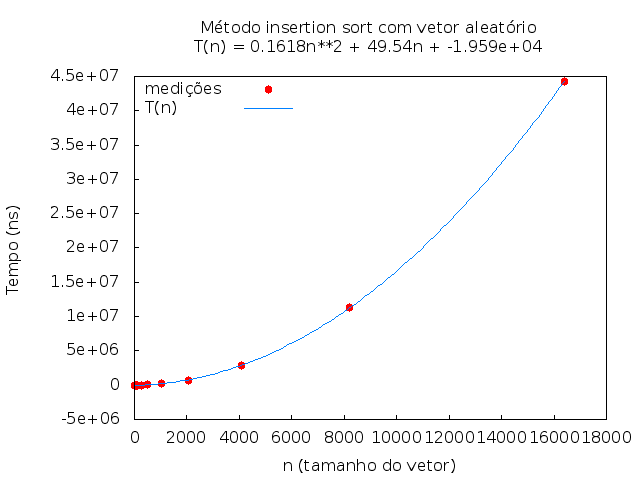
\includegraphics[width=0.7\linewidth]{graficos/Insertion/vIntAleatorio/vIntAleatorio.png}
  \caption{Gráfico Insertion Sort - Vetor Aleatorio}
\end{figure}


\section{Insertion Sort - Vetor Crescente}
Tabela gerada utilizando Insertion Sort com vetores de tamanho n, sendo = $(2^k)$, k = 4...14 e inseridos em ordem crescente.

\begin{table}[H]
\centering
\caption{Insertion Sort com Vetor ordenado em ordem crescente}
\label{my-label}
\begin{tabular}{|l|l|}
\hline
\multicolumn{1}{|c|}{\textbf{Número de Elementos}} & \multicolumn{1}{c|}{\textbf{Tempo de execução em nanosegundos}} \\ \hline
16 & 330 \\ \hline
32 & 359 \\ \hline
64 & 366 \\ \hline
128 & 441 \\ \hline
256 & 653 \\ \hline
512 & 1151 \\ \hline
1024 & 1616 \\ \hline
2048 & 3006 \\ \hline
4096 & 5551 \\ \hline
8192 & 11105 \\ \hline
16384 & 21993 \\ \hline
\end{tabular}
\end{table}

\subsection{Grafico Insertion Sort - Vetor Crescente}
\begin{figure}[H]
    \centering
    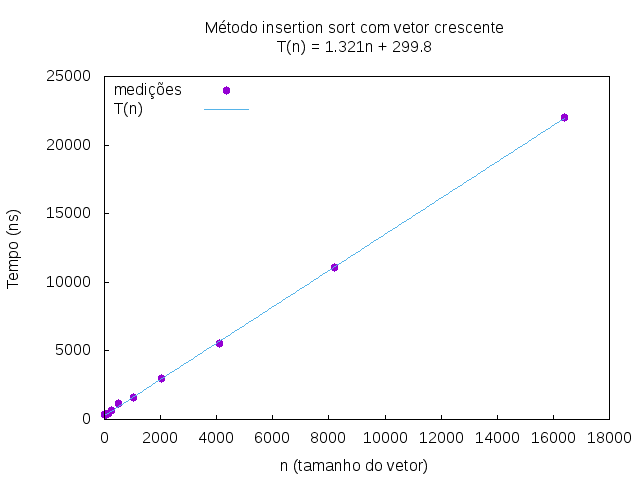
\includegraphics[width=0.7\linewidth]{graficos/Insertion/vIntCrescente/vIntCrescente.png}
  \caption{Gráfico Insertion Sort - Vetor Crescente}
\end{figure}

\section{Insertion Sort - Vetor Crescente P10}
Tabela gerada utilizando Insertion Sort com vetores de tamanho n, sendo = $(2^k)$, k = 4...14 e inseridos em ordem crescente estando 10\% ordenado.

\begin{table}[H]
\centering
\caption{Insertion Sort com Vetor ordenado em ordem crescente 10\% ordenado}
\label{my-label}
\begin{tabular}{|l|l|}
\hline
\multicolumn{1}{|c|}{\textbf{Número de Elementos}} & \multicolumn{1}{c|}{\textbf{Tempo de execução em nanosegundos}} \\ \hline
16 & 306 \\ \hline
32 & 401 \\ \hline
64 & 641 \\ \hline
128 & 1477 \\ \hline
256 & 4722 \\ \hline
512 & 17262 \\ \hline
1024 & 73246 \\ \hline
2048 & 304783 \\ \hline
4096 & 1140882 \\ \hline
8192 & 4421923 \\ \hline
16384 & 17366826 \\ \hline
\end{tabular}
\end{table}

\subsection{Grafico Insertion Sort - Vetor Crescente P10}
\begin{figure}[H]
    \centering
    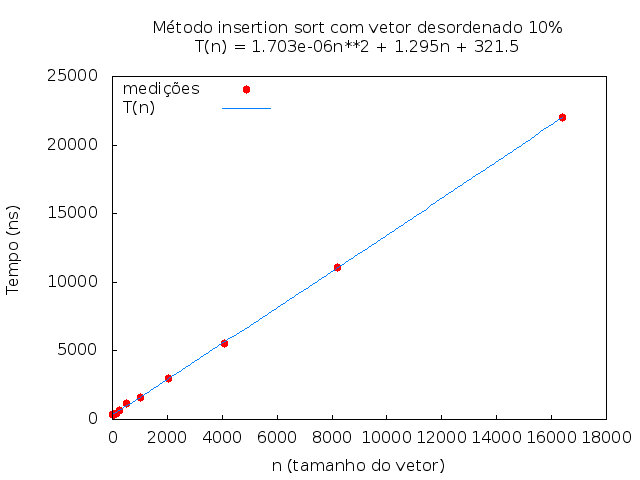
\includegraphics[width=0.7\linewidth]{graficos/Insertion/vIntCrescenteP10/vIntCrescenteP10.png}
  \caption{Gráfico Insertion Sort - Vetor Crescente P10}
\end{figure}

\section{Insertion Sort - Vetor Crescente P20}
Tabela gerada utilizando Insertion Sort com vetores de tamanho n, sendo = $(2^k)$, k = 4...14 e inseridos em ordem crescente estando 20\% ordenado.

\begin{table}[H]
\centering
\caption{Insertion Sort com Vetor ordenado em ordem crescente 20\% ordenado}
\label{my-label}
\begin{tabular}{|l|l|}
\hline
\multicolumn{1}{|c|}{\textbf{Número de Elementos}} & \multicolumn{1}{c|}{\textbf{Tempo de execução em nanosegundos}} \\ \hline
16 & 395 \\ \hline
32 & 528 \\ \hline
64 & 942 \\ \hline
128 & 2441 \\ \hline
256 & 8518 \\ \hline
512 & 37766 \\ \hline
1024 & 188395 \\ \hline
2048 & 561783 \\ \hline
4096 & 2024058 \\ \hline
8192 & 8326582 \\ \hline
16384 & 32720219 \\ \hline
\end{tabular}
\end{table}

\subsection{Grafico Insertion Sort - Vetor Crescente P20}
\begin{figure}[H]
    \centering
    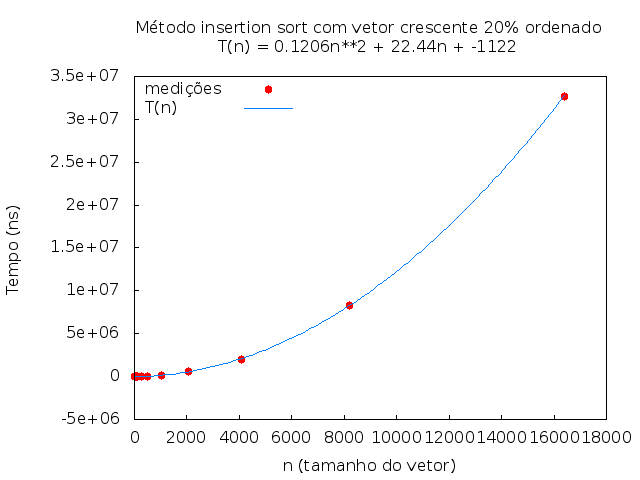
\includegraphics[width=0.7\linewidth]{graficos/Insertion/vIntCrescenteP20/vIntCrescenteP20.png}
  \caption{Gráfico Insertion Sort - Vetor Crescente P20}
\end{figure}


\section{Insertion Sort - Vetor Crescente P30}
Tabela gerada utilizando Insertion Sort com vetores de tamanho n, sendo = $(2^k)$, k = 4...14 e inseridos em ordem crescente estando 30\% ordenado.

\begin{table}[H]
\centering
\caption{Insertion Sort com Vetor ordenado em ordem crescente 30\% ordenado}
\label{my-label}
\begin{tabular}{|l|l|}
\hline
\multicolumn{1}{|c|}{\textbf{Número de Elementos}} & \multicolumn{1}{c|}{\textbf{Tempo de execução em nanosegundos}} \\ \hline
16 & 426 \\ \hline
32 & 565 \\ \hline
64 & 1121 \\ \hline
128 & 3639 \\ \hline
256 & 11877 \\ \hline
512 & 47210 \\ \hline
1024 & 188411 \\ \hline
2048 & 747231 \\ \hline
4096 & 2903599 \\ \hline
8192 & 11706837 \\ \hline
16384 & 46407450 \\ \hline
\end{tabular}
\end{table}

\subsection{Grafico Insertion Sort - Vetor Crescente P30}
\begin{figure}[H]
    \centering
    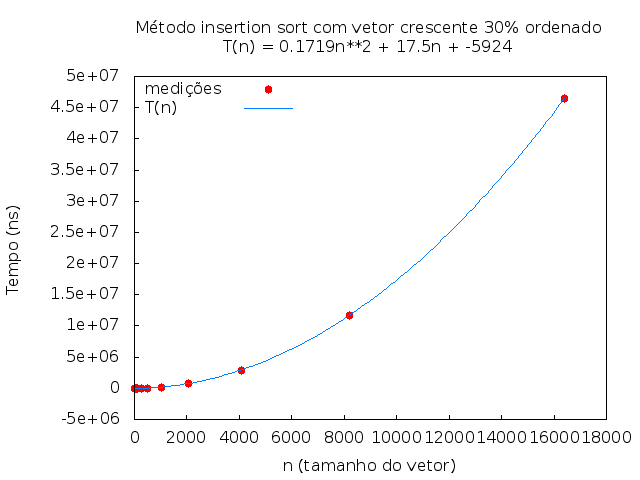
\includegraphics[width=0.7\linewidth]{graficos/Insertion/vIntCrescenteP30/vIntCrescenteP30.png}
  \caption{Gráfico Insertion Sort - Vetor Crescente P30}
\end{figure}


\section{Insertion Sort - Vetor Crescente P40}
Tabela gerada utilizando Insertion Sort com vetores de tamanho n, sendo = $(2^k)$, k = 4...14 e inseridos em ordem crescente estando 40\% ordenado.

\begin{table}[H]
\centering
\caption{Insertion Sort com Vetor ordenado em ordem crescente 40\% ordenado}
\label{my-label}
\begin{tabular}{|l|l|}
\hline
\multicolumn{1}{|c|}{\textbf{Número de Elementos}} & \multicolumn{1}{c|}{\textbf{Tempo de execução em nanosegundos}} \\ \hline
16 & 419 \\ \hline
32 & 587 \\ \hline
64 & 1308 \\ \hline
128 & 4090 \\ \hline
256 & 15835 \\ \hline
512 & 65553 \\ \hline
1024 & 224888 \\ \hline
2048 & 916018 \\ \hline
4096 & 3680777 \\ \hline
8192 & 14947212 \\ \hline
16384 & 59251527 \\ \hline
\end{tabular}
\end{table}

\subsection{Grafico Insertion Sort - Vetor Crescente P40}
\begin{figure}[H]
    \centering
    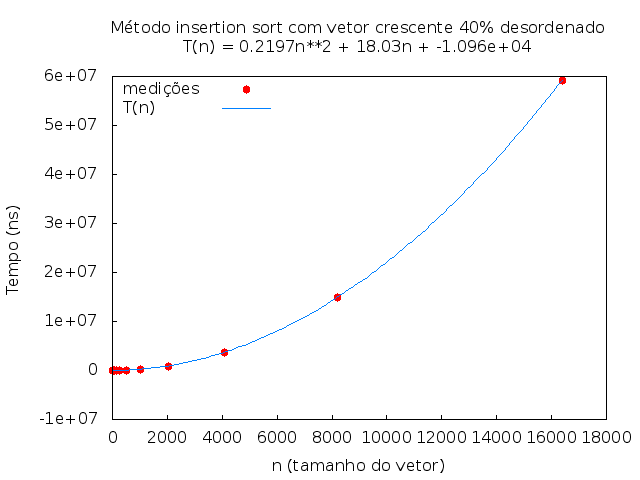
\includegraphics[width=0.7\linewidth]{graficos/Insertion/vIntCrescenteP40/vIntCrescenteP40.png}
  \caption{Gráfico Insertion Sort - Vetor Crescente P40}
\end{figure}


\section{Insertion Sort - Vetor Crescente P50}
Tabela gerada utilizando Insertion Sort com vetores de tamanho n, sendo = $(2^k)$, k = 4...14 e inseridos em ordem crescente estando 50\% ordenado.

\begin{table}[H]
\centering
\caption{Insertion Sort com Vetor ordenado em ordem crescente 50\% ordenado}
\label{my-label}
\begin{tabular}{|l|l|}
\hline
\multicolumn{1}{|c|}{\textbf{Número de Elementos}} & \multicolumn{1}{c|}{\textbf{Tempo de execução em nanosegundos}} \\ \hline
16 & 558 \\ \hline
32 & 659 \\ \hline
64 & 1513 \\ \hline
128 & 17337 \\ \hline
256 & 18190 \\ \hline
512 & 67937 \\ \hline
1024 & 262668 \\ \hline
2048 & 1100335 \\ \hline
4096 & 4360290 \\ \hline
8192 & 17429716 \\ \hline
16384 & 67965063 \\ \hline
\end{tabular}
\end{table}

\subsection{Grafico Insertion Sort - Vetor Crescente P50}
\begin{figure}[H]
    \centering
    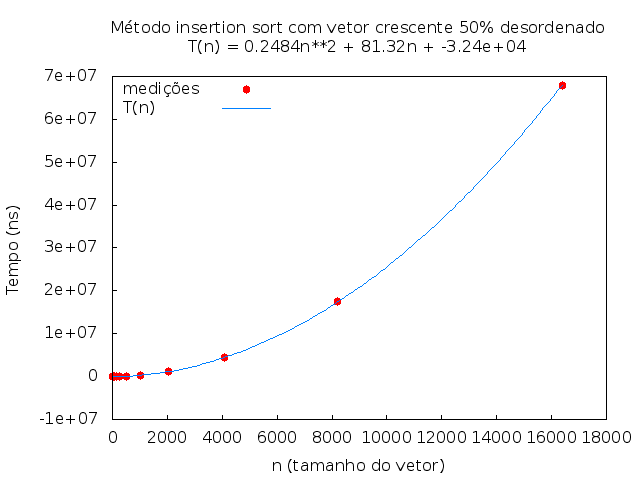
\includegraphics[width=0.7\linewidth]{graficos/Insertion/vIntCrescenteP50/vIntCrescenteP50.png}
  \caption{Gráfico Insertion Sort - Vetor Crescente P50}
\end{figure}


\section{Insertion Sort - Vetor Decrescente}
Tabela gerada utilizando Insertion Sort com vetores de tamanho n, sendo = $(2^k)$, k = 4...14 e inseridos em ordem decrescente.

\begin{table}[H]
\centering
\caption{Insertion Sort com Vetor ordenado em ordem decrescente}
\label{my-label}
\begin{tabular}{|l|l|}
\hline
\multicolumn{1}{|c|}{\textbf{Número de Elementos}} & \multicolumn{1}{c|}{\textbf{Tempo de execução em nanosegundos}} \\ \hline
16 & 755 \\ \hline
32 & 874 \\ \hline
64 & 2328 \\ \hline
128 & 7374 \\ \hline
256 & 24763 \\ \hline
512 & 93192 \\ \hline
1024 & 348188 \\ \hline
2048 & 1395270 \\ \hline
4096 & 5750603 \\ \hline
8192 & 24268503 \\ \hline
16384 & 95007321 \\ \hline
\end{tabular}
\end{table}

\subsection{Grafico Insertion Sort - Vetor Decrescente}
\begin{figure}[H]
    \centering
    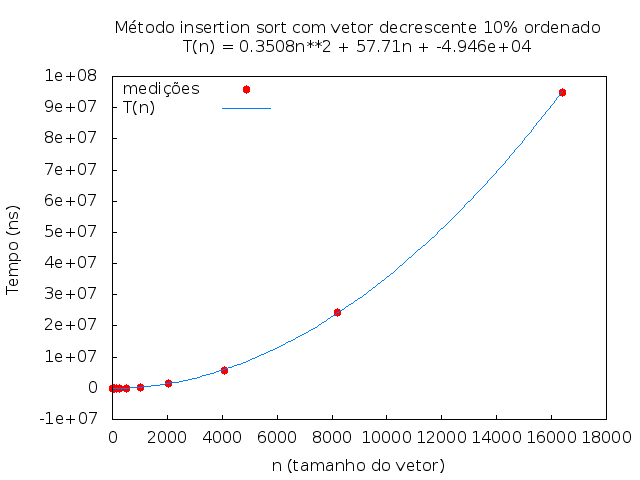
\includegraphics[width=0.7\linewidth]{graficos/Insertion/vIntDecrescente/vIntDecrescente.png}
  \caption{Gráfico Insertion Sort - Vetor Decrescente}
\end{figure}


\section{Insertion Sort - Vetor Decrescente P10}
Tabela gerada utilizando Insertion Sort com vetores de tamanho n, sendo = $(2^k)$, k = 4...14 e inseridos em ordem descrescente estando 10\% ordenado.

\begin{table}[H]
\centering
\caption{Insertion Sort com Vetor ordenado em ordem descrecente 10\% ordenado}
\label{my-label}
\begin{tabular}{|l|l|}
\hline
\multicolumn{1}{|c|}{\textbf{Número de Elementos}} & \multicolumn{1}{c|}{\textbf{Tempo de execução em nanosegundos}} \\ \hline
16 & 458 \\ \hline
32 & 875 \\ \hline
64 & 1835 \\ \hline
128 & 5721 \\ \hline
256 & 19634 \\ \hline
512 & 73075 \\ \hline
1024 & 296395 \\ \hline
2048 & 1193812 \\ \hline
4096 & 4766396 \\ \hline
8192 & 19593295 \\ \hline
16384 & 77500644 \\ \hline
\end{tabular}
\end{table}

\subsection{Grafico Insertion Sort - Vetor Decrescente P10}
\begin{figure}[H]
    \centering
    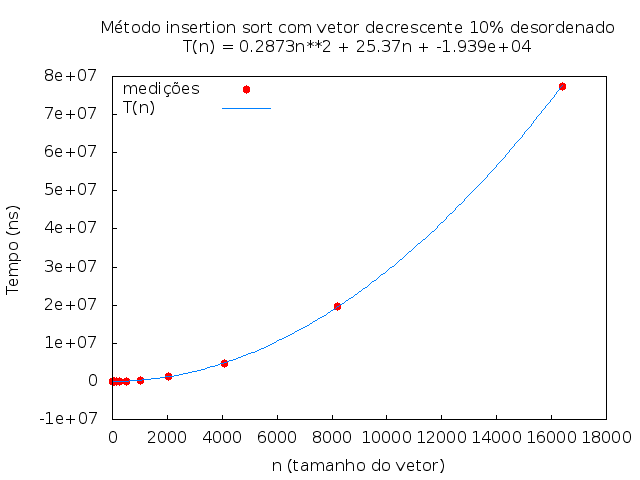
\includegraphics[width=0.7\linewidth]{graficos/Insertion/vIntDecrescenteP10/vIntDecrescenteP10.png}
  \caption{Gráfico Insertion Sort - Vetor Decrescente P10}
\end{figure}

\section{Insertion Sort - Vetor Decrescente P20}
Tabela gerada utilizando Insertion Sort com vetores de tamanho n, sendo = $(2^k)$, k = 4...14 e inseridos em ordem descrescente estando 20\% ordenado.

\begin{table}[H]
\centering
\caption{Insertion Sort com Vetor ordenado em ordem descrecente 20\% ordenado}
\label{my-label}
\begin{tabular}{|l|l|}
\hline
\multicolumn{1}{|c|}{\textbf{Número de Elementos}} & \multicolumn{1}{c|}{\textbf{Tempo de execução em nanosegundos}} \\ \hline
16 & 486 \\ \hline
32 & 667 \\ \hline
64 & 1535 \\ \hline
128 & 4529 \\ \hline
256 & 15714 \\ \hline
512 & 58010 \\ \hline
1024 & 230754 \\ \hline
2048 & 906191 \\ \hline
4096 & 4298422 \\ \hline
8192 & 15435783 \\ \hline
16384 & 59268139 \\ \hline
\end{tabular}
\end{table}

\subsection{Grafico Insertion Sort - Vetor Decrescente P20}
\begin{figure}[H]
    \centering
    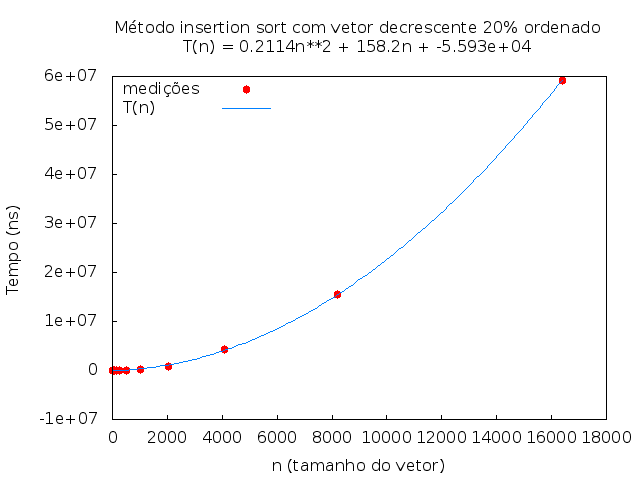
\includegraphics[width=0.7\linewidth]{graficos/Insertion/vIntDecrescenteP20/vIntDecrescenteP20.png}
  \caption{Gráfico Insertion Sort - Vetor Decrescente P20}
\end{figure}

\section{Insertion Sort - Vetor Decrescente P30}
Tabela gerada utilizando Insertion Sort com vetores de tamanho n, sendo = $(2^k)$, k = 4...14 e inseridos em ordem descrescente estando 30\% ordenado.

\begin{table}[H]
\centering
\caption{Insertion Sort com Vetor ordenado em ordem descrecente 30\% ordenado}
\label{my-label}
\begin{tabular}{|l|l|}
\hline
\multicolumn{1}{|c|}{\textbf{Número de Elementos}} & \multicolumn{1}{c|}{\textbf{Tempo de execução em nanosegundos}} \\ \hline
16 & 472 \\ \hline
32 & 618 \\ \hline
64 & 1315 \\ \hline
128 & 3584 \\ \hline
256 & 12212 \\ \hline
512 & 45720 \\ \hline
1024 & 176462 \\ \hline
2048 & 713725 \\ \hline
4096 & 2722869 \\ \hline
8192 & 11098439 \\ \hline
16384 & 43472556 \\ \hline
\end{tabular}
\end{table}

\subsection{Grafico Insertion Sort - Vetor Decrescente P30}
\begin{figure}[H]
    \centering
    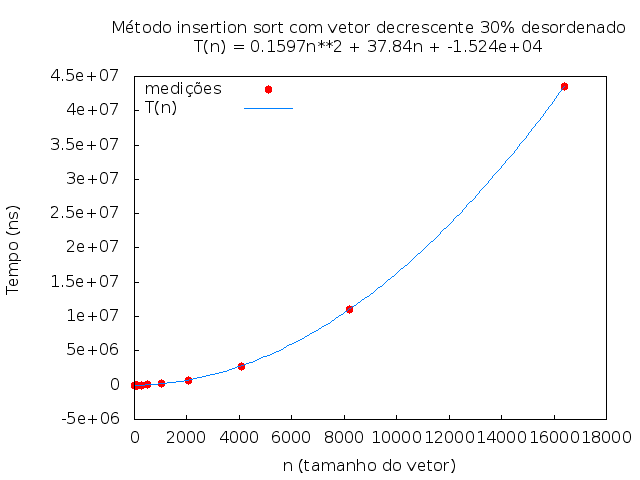
\includegraphics[width=0.7\linewidth]{graficos/Insertion/vIntDecrescenteP30/vIntDecrescenteP30.png}
  \caption{Gráfico Insertion Sort - Vetor Decrescente P30}
\end{figure}


\section{Insertion Sort - Vetor Decrescente P40}
Tabela gerada utilizando Insertion Sort com vetores de tamanho n, sendo = $(2^k)$, k = 4...14 e inseridos em ordem descrescente estando 40\% ordenado.

\begin{table}[H]
\centering
\caption{Insertion Sort com Vetor ordenado em ordem descrecente 40\% ordenado}
\label{my-label}
\begin{tabular}{|l|l|}
\hline
\multicolumn{1}{|c|}{\textbf{Número de Elementos}} & \multicolumn{1}{c|}{\textbf{Tempo de execução em nanosegundos}} \\ \hline
16 & 455 \\ \hline
32 & 617 \\ \hline
64 & 1161 \\ \hline
128 & 5847 \\ \hline
256 & 8949 \\ \hline
512 & 32581 \\ \hline
1024 & 135069 \\ \hline
2048 & 503857 \\ \hline
4096 & 2004770 \\ \hline
8192 & 8252574 \\ \hline
16384 & 31871258 \\ \hline
\end{tabular}
\end{table}

\subsection{Grafico Insertion Sort - Vetor Decrescente P40}
\begin{figure}[H]
    \centering
    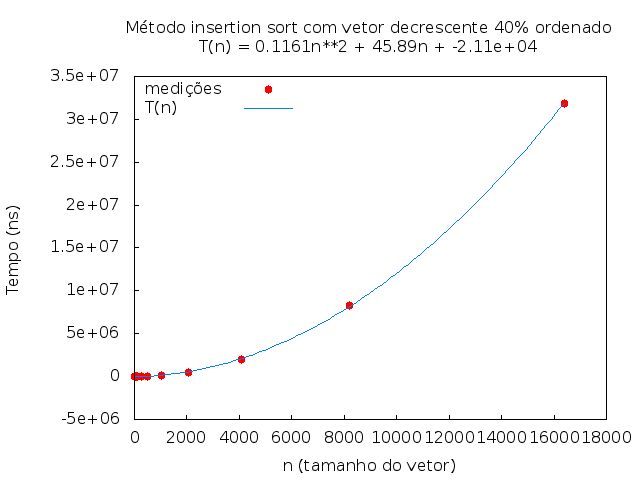
\includegraphics[width=0.7\linewidth]{graficos/Insertion/vIntDecrescenteP40/vIntDecrescenteP40.png}
  \caption{Gráfico Insertion Sort - Vetor Decrescente P40}
\end{figure}


\section{Insertion Sort - Vetor Decrescente P50}
Tabela gerada utilizando Insertion Sort com vetores de tamanho n, sendo = $(2^k)$, k = 4...14 e inseridos em ordem descrescente estando 50\% ordenado.

\begin{table}[H]
\centering
\caption{Insertion Sort com Vetor ordenado em ordem descrecente 50\% ordenado}
\label{my-label}
\begin{tabular}{|l|l|}
\hline
\multicolumn{1}{|c|}{\textbf{Número de Elementos}} & \multicolumn{1}{c|}{\textbf{Tempo de execução em nanosegundos}} \\ \hline
16 & 409 \\ \hline
32 & 461 \\ \hline
64 & 847 \\ \hline
128 & 2144 \\ \hline
256 & 6683 \\ \hline
512 & 23838 \\ \hline
1024 & 89838 \\ \hline
2048 & 352101 \\ \hline
4096 & 1389637 \\ \hline
8192 & 5639428 \\ \hline
16384 & 22348219 \\ \hline
\end{tabular}
\end{table}

\subsection{Grafico Insertion Sort - Vetor Decrescente P50}
\begin{figure}[H]
    \centering
    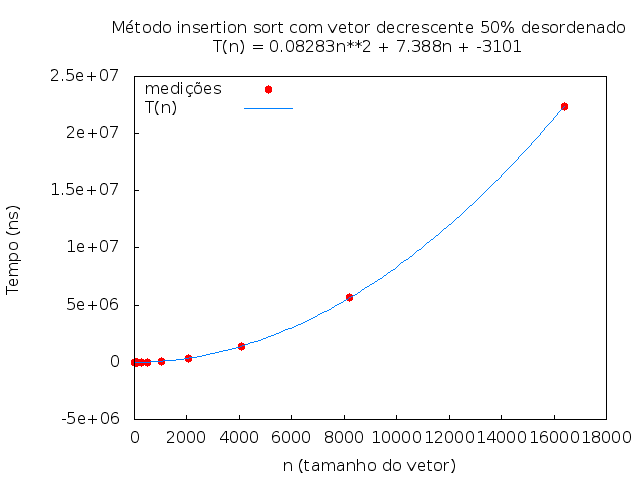
\includegraphics[width=0.7\linewidth]{graficos/Insertion/vIntDecrescenteP50/vIntDecrescenteP50.png}
  \caption{Gráfico Insertion Sort - Vetor Decrescente P50}
\end{figure}

\section{Observações Finais}
Insertion em ordem decrescente com $2^k$ com k = 32 elementos: levaria aproximadamente 205 anos e 22 dias 

\chapter{Merge Sort}
O algoritmo de ordenação Merge Sort (Intercalação) ordena por comparações utilizando o conceito de dividir-para-conquistar.
Basicamente o algoritmo divide o problema em vários sub-problemas e os resolve através de recursividade e conquista pegando o unindo todos os sub-problemas que foram resolvidos.
Em qualquer caso, temos que o algoritmo MergeSort tem complexidade de tempo $\theta(nlogn)$.

\section{Merge Sort - Vetor Aleatório}
Tabela gerada utilizando Merge Sort com vetores de tamanho n, sendo n = $(2^k)$, de k = 4..14 e inseridos aleatóriamente.
\begin{table}[H]
\centering
\caption{Merge Sort com vetor aleatório}
\label{my-label}
\begin{tabular}{|l|l|}
\hline
\multicolumn{1}{|c|}{\textbf{Número de Elementos}} & \multicolumn{1}{c|}{\textbf{Tempo de execução em nanosegundos}} \\ \hline
16 & 2761 \\ \hline
32 & 3438 \\ \hline
64 & 7886 \\ \hline
128 & 16043 \\ \hline
256 & 33294 \\ \hline
512 & 75211 \\ \hline
1024 & 186557 \\ \hline
2048 & 477554 \\ \hline
4096 & 1278453 \\ \hline
8192 & 4144242 \\ \hline
16384 & 18189873 \\ \hline
\end{tabular}
\end{table}

\subsection{Gráfico Merge Sort - Vetor Aleatório}
\begin{figure}[H]
    \centering
    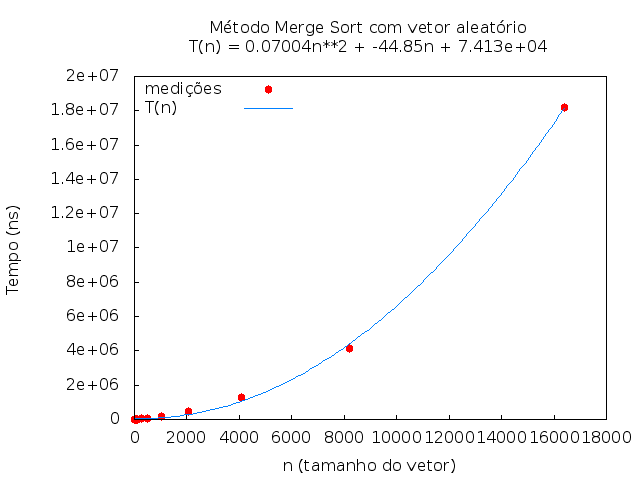
\includegraphics[width=0.7\linewidth]{graficos/MergeSort/vIntAleatorio/vIntAleatorio.png}
  \caption{Gráfico Merge Sort - Vetor Aleatório}
\end{figure}

\section{Merge Sort - Vetor Crescente}
Tabela gerada utilizando Merge Sort com vetores de tamanho n, sendo n = $(2^k)$, de k = 4..14 e inseridos em ordem crescente.
\begin{table}[H]
\centering
\caption{Merge Sort com vetor ordenado em ordem crescente}
\label{my-label}
\begin{tabular}{|l|l|}
\hline
\multicolumn{1}{|c|}{\textbf{Número de Elementos}} & \multicolumn{1}{c|}{\textbf{Tempo de execução em nanosegundos}} \\ \hline
16 & 1840 \\ \hline
32 & 3284 \\ \hline
64 & 6768 \\ \hline
128 & 13027 \\ \hline
256 & 26564 \\ \hline
512 & 59916 \\ \hline
1024 & 144530 \\ \hline
2048 & 368955 \\ \hline
4096 & 1095195 \\ \hline
8192 & 3812048 \\ \hline
16384 & 17545434 \\ \hline
\end{tabular}
\end{table}

\subsection{Gráfico Merge Sort - Vetor Crescente}
\begin{figure}[H]
    \centering
    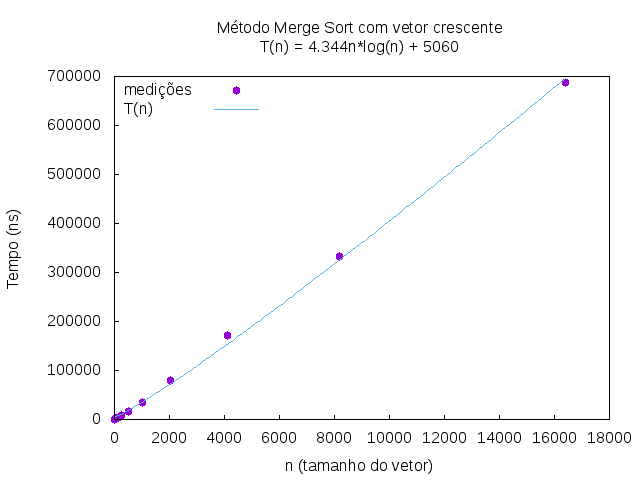
\includegraphics[width=0.7\linewidth]{graficos/MergeSort/vIntCrescente/vIntCrescente.png}
  \caption{Gráfico Merge Sort - Vetor Crescente}
\end{figure}

\section{Merge Sort - Vetor Crescente P10}
Tabela gerada utilizando Merge Sort com vetores de tamanho n, sendo n = $(2^k)$, de k = 4..14 e inseridos em ordem crescente estando 10\% ordenado.
\begin{table}[H]
\centering
\caption{Merge Sort com vetor ordenado em ordem crescente estando 10\% ordenado}
\label{my-label}
\begin{tabular}{|l|l|}
\hline
\multicolumn{1}{|c|}{\textbf{Número de Elementos}} & \multicolumn{1}{c|}{\textbf{Tempo de execução em nanosegundos}} \\ \hline
16 & 1732 \\ \hline
32 & 3328 \\ \hline
64 & 6776 \\ \hline
128 & 12591 \\ \hline
256 & 30350 \\ \hline
512 & 65121 \\ \hline
1024 & 150315 \\ \hline
2048 & 367101 \\ \hline
4096 & 1105073 \\ \hline
8192 & 3896594 \\ \hline
16384 & 17300648 \\ \hline
\end{tabular}
\end{table}

\subsection{Gráfico Merge Sort - Vetor Crescente P10}
\begin{figure}[H]
    \centering
    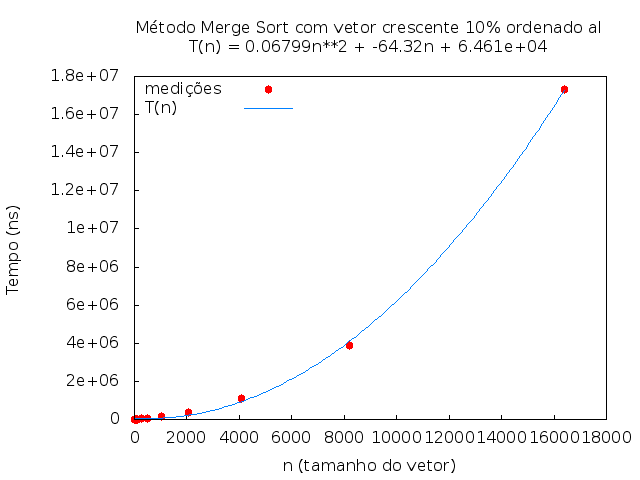
\includegraphics[width=0.7\linewidth]{graficos/MergeSort/vIntCrescenteP10/vIntCrescenteP10.png}
  \caption{Gráfico Merge Sort - Vetor Crescente P10}
\end{figure}

\section{Merge Sort - Vetor Crescente P20}
Tabela gerada utilizando Merge Sort com vetores de tamanho n, sendo n = $(2^k)$, de k = 4..14 e inseridos em ordem crescente estando 20\% ordenado.
\begin{table}[H]
\centering
\caption{Merge Sort com vetor ordenado em ordem crescente estando 20\% ordenado}
\label{my-label}
\begin{tabular}{|l|l|}
\hline
\multicolumn{1}{|c|}{\textbf{Número de Elementos}} & \multicolumn{1}{c|}{\textbf{Tempo de execução em nanosegundos}} \\ \hline
16 & 1789 \\ \hline
32 & 3337 \\ \hline
64 & 6866 \\ \hline
128 & 12755 \\ \hline
256 & 29327 \\ \hline
512 & 63476 \\ \hline
1024 & 148528 \\ \hline
2048 & 367361 \\ \hline
4096 & 1072801 \\ \hline
8192 & 3846028 \\ \hline
16384 & 17413999 \\ \hline
\end{tabular}
\end{table}

\subsection{Gráfico Merge Sort - Vetor Crescente P20}
\begin{figure}[H]
    \centering
    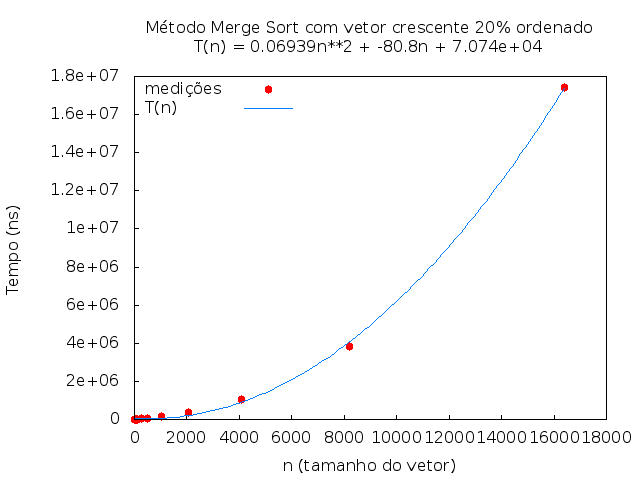
\includegraphics[width=0.7\linewidth]{graficos/MergeSort/vIntCrescenteP20/vIntCrescenteP20.png}
  \caption{Gráfico Merge Sort - Vetor Crescente P20}
\end{figure}

\section{Merge Sort - Vetor Crescente P30}
Tabela gerada utilizando Merge Sort com vetores de tamanho n, sendo n = $(2^k)$, de k = 4..14 e inseridos em ordem crescente estando 30\% ordenado.
\begin{table}[H]
\centering
\caption{Merge Sort com vetor ordenado em ordem crescente estando 30\% ordenado}
\label{my-label}
\begin{tabular}{|l|l|}
\hline
\multicolumn{1}{|c|}{\textbf{Número de Elementos}} & \multicolumn{1}{c|}{\textbf{Tempo de execução em nanosegundos}} \\ \hline
16 & 2042 \\ \hline
32 & 3304 \\ \hline
64 & 6831 \\ \hline
128 & 14759 \\ \hline
256 & 28846 \\ \hline
512 & 62768 \\ \hline
1024 & 147870 \\ \hline
2048 & 362086 \\ \hline
4096 & 1072534 \\ \hline
8192 & 3822915 \\ \hline
16384 & 17393637 \\ \hline
\end{tabular}
\end{table}

\subsection{Gráfico Merge Sort - Vetor Crescente P30}
\begin{figure}[H]
    \centering
    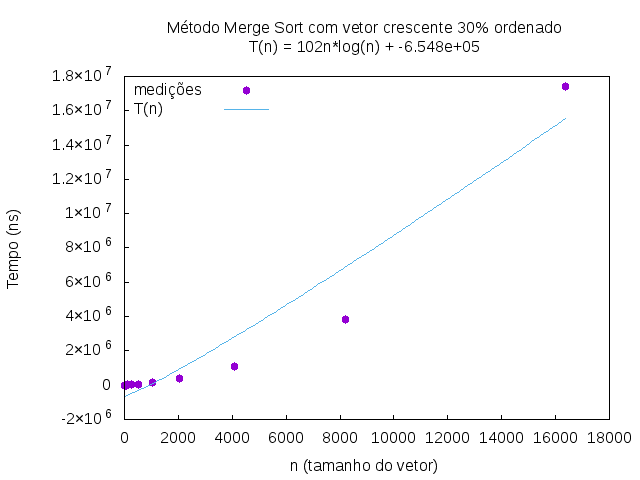
\includegraphics[width=0.7\linewidth]{graficos/MergeSort/vIntCrescenteP30/vIntCrescenteP30.png}
  \caption{Gráfico Merge Sort - Vetor Crescente P30}
\end{figure}

\section{Merge Sort - Vetor Crescente P40}
Tabela gerada utilizando Merge Sort com vetores de tamanho n, sendo n = $(2^k)$, de k = 4..14 e inseridos em ordem crescente estando 40\% ordenado.
\begin{table}[H]
\centering
\caption{Merge Sort com vetor ordenado em ordem crescente estando 40\% ordenado}
\label{my-label}
\begin{tabular}{|l|l|}
\hline
\multicolumn{1}{|c|}{\textbf{Número de Elementos}} & \multicolumn{1}{c|}{\textbf{Tempo de execução em nanosegundos}} \\ \hline
16 & 1951 \\ \hline
32 & 3272 \\ \hline
64 & 6625 \\ \hline
128 & 12620 \\ \hline
256 & 28417 \\ \hline
512 & 66034 \\ \hline
1024 & 151603 \\ \hline
2048 & 366825 \\ \hline
4096 & 1077138 \\ \hline
8192 & 3950780 \\ \hline
16384 & 17461202 \\ \hline
\end{tabular}
\end{table}

\subsection{Gráfico Merge Sort - Vetor Crescente P40}
\begin{figure}[H]
    \centering
    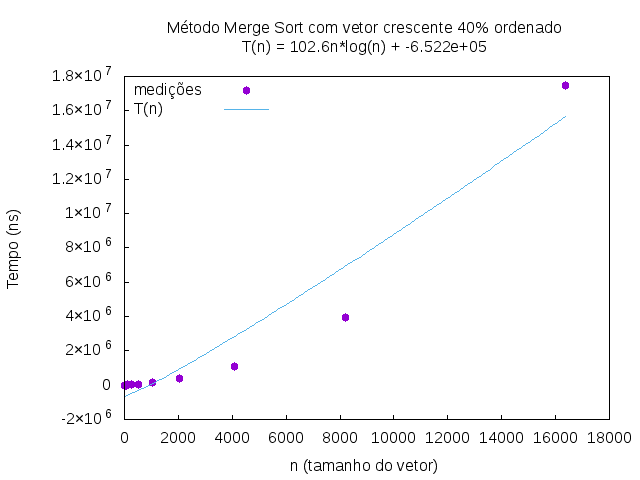
\includegraphics[width=0.7\linewidth]{graficos/MergeSort/vIntCrescenteP40/vIntCrescenteP40.png}
  \caption{Gráfico Merge Sort - Vetor Crescente P40}
\end{figure}

\section{Merge Sort - Vetor Crescente P50}
Tabela gerada utilizando Merge Sort com vetores de tamanho n, sendo n = $(2^k)$, de k = 4..14 e inseridos em ordem crescente estando 50\% ordenado.
\begin{table}[H]
\centering
\caption{Merge Sort com vetor ordenado em ordem crescente estando 50\% ordenado}
\label{my-label}
\begin{tabular}{|l|l|}
\hline
\multicolumn{1}{|c|}{\textbf{Número de Elementos}} & \multicolumn{1}{c|}{\textbf{Tempo de execução em nanosegundos}} \\ \hline
16 & 1850 \\ \hline
32 & 3506 \\ \hline
64 & 6465 \\ \hline
128 & 12959 \\ \hline
256 & 28681 \\ \hline
512 & 62483 \\ \hline
1024 & 146989 \\ \hline
2048 & 365252 \\ \hline
4096 & 1076419 \\ \hline
8192 & 3951343 \\ \hline
16384 & 17351729 \\ \hline
\end{tabular}
\end{table}

\subsection{Gráfico Merge Sort - Vetor Crescente P50}
\begin{figure}[H]
    \centering
    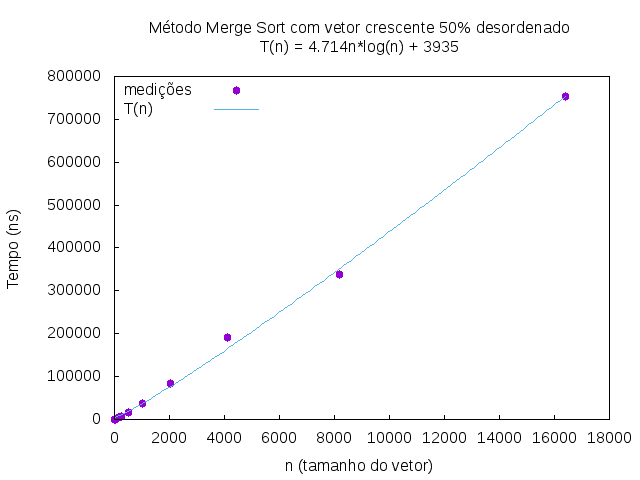
\includegraphics[width=0.7\linewidth]{graficos/MergeSort/vIntCrescenteP50/vIntCrescenteP50.png}
  \caption{Gráfico Merge Sort - Vetor Crescente P50}
\end{figure}

\section{Merge Sort - Vetor Decrescente}
Tabela gerada utilizando Merge Sort com vetores de tamanho n, sendo n = $(2^k)$, de k = 4..14 e inseridos em ordem decrescente.
\begin{table}[H]
\centering
\caption{Merge Sort com vetor ordenado em ordem decrescente}
\label{my-label}
\begin{tabular}{|l|l|}
\hline
\multicolumn{1}{|c|}{\textbf{Número de Elementos}} & \multicolumn{1}{c|}{\textbf{Tempo de execução em nanosegundos}} \\ \hline
16 & 1969 \\ \hline
32 & 3171 \\ \hline
64 & 6247 \\ \hline
128 & 12520 \\ \hline
256 & 27287 \\ \hline
512 & 83363 \\ \hline
1024 & 145250 \\ \hline
2048 & 369093 \\ \hline
4096 & 1066356 \\ \hline
8192 & 3968570 \\ \hline
16384 & 17262377 \\ \hline
\end{tabular}
\end{table}

\subsection{Gráfico Merge Sort - Vetor Decrescente}
\begin{figure}[H]
    \centering
    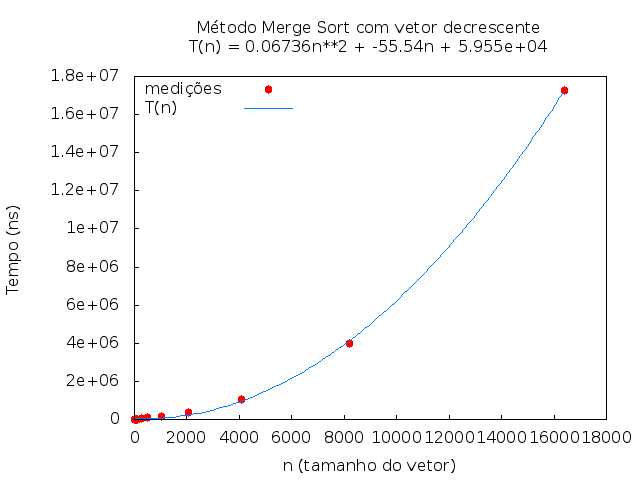
\includegraphics[width=0.7\linewidth]{graficos/MergeSort/vIntDecrescente/vIntDecrescente.png}
  \caption{Gráfico Merge Sort - Vetor Decrescente}
\end{figure}

\section{Merge Sort - Vetor Decrescente P10}
Tabela gerada utilizando Merge Sort com vetores de tamanho n, sendo n = $(2^k)$, de k = 4..14 e inseridos em ordem decrescente estando 10\% ordenado.
\begin{table}[H]
\centering
\caption{Merge Sort com vetor ordenado em ordem decrescente estando 10\% ordenado}
\label{my-label}
\begin{tabular}{|l|l|}
\hline
\multicolumn{1}{|c|}{\textbf{Número de Elementos}} & \multicolumn{1}{c|}{\textbf{Tempo de execução em nanosegundos}} \\ \hline
16 & 1915 \\ \hline
32 & 3234 \\ \hline
64 & 6637 \\ \hline
128 & 12565 \\ \hline
256 & 33715 \\ \hline
512 & 62647 \\ \hline
1024 & 157201 \\ \hline
2048 & 363791 \\ \hline
4096 & 1069486 \\ \hline
8192 & 3941973 \\ \hline
16384 & 17409501 \\ \hline
\end{tabular}
\end{table}

\subsection{Gráfico Merge Sort - Vetor Decrescente P10}
\begin{figure}[H]
    \centering
    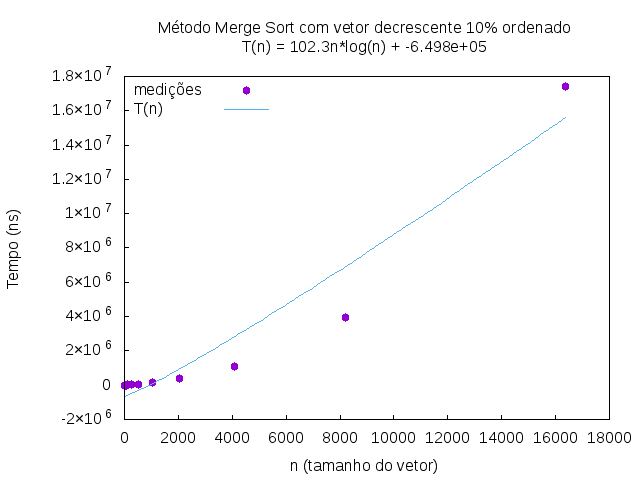
\includegraphics[width=0.7\linewidth]{graficos/MergeSort/vIntDecrescenteP10/vIntDecrescenteP10.png}
  \caption{Gráfico Merge Sort - Vetor Decrescente P10}
\end{figure}

\section{Merge Sort - Vetor Decrescente P20}
Tabela gerada utilizando Merge Sort com vetores de tamanho n, sendo n = $(2^k)$, de k = 4..14 e inseridos em ordem decrescente estando 20\% ordenado.
\begin{table}[H]
\centering
\caption{Merge Sort com vetor ordenado em ordem decrescente estando 20\% ordenado}
\label{my-label}
\begin{tabular}{|l|l|}
\hline
\multicolumn{1}{|c|}{\textbf{Número de Elementos}} & \multicolumn{1}{c|}{\textbf{Tempo de execução em nanosegundos}} \\ \hline
16 & 2093 \\ \hline
32 & 3162 \\ \hline
64 & 6737 \\ \hline
128 & 12671 \\ \hline
256 & 34914 \\ \hline
512 & 62345 \\ \hline
1024 & 151220 \\ \hline
2048 & 373987 \\ \hline
4096 & 1082704 \\ \hline
8192 & 3849662 \\ \hline
16384 & 17495764 \\ \hline
\end{tabular}
\end{table}

\subsection{Gráfico Merge Sort - Vetor Decrescente P20}
\begin{figure}[H]
    \centering
    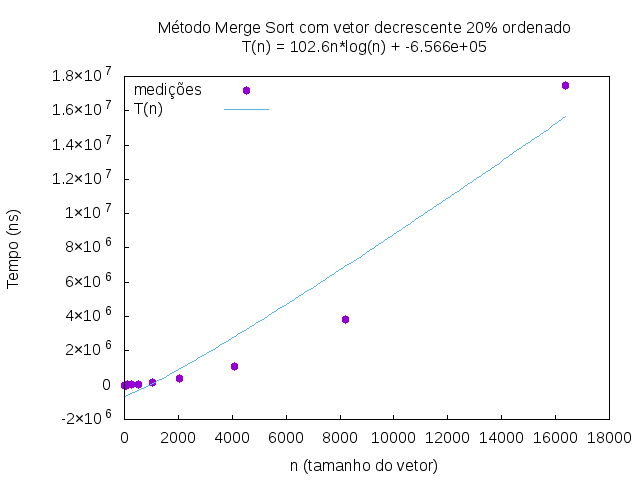
\includegraphics[width=0.7\linewidth]{graficos/MergeSort/vIntDecrescenteP20/vIntDecrescenteP20.png}
  \caption{Gráfico Merge Sort - Vetor Decrescente P20}
\end{figure}

\section{Merge Sort - Vetor Decrescente P30}
Tabela gerada utilizando Merge Sort com vetores de tamanho n, sendo n = $(2^k)$, de k = 4..14 e inseridos em ordem decrescente estando 30\% ordenado.
\begin{table}[H]
\centering
\caption{Merge Sort com vetor ordenado em ordem decrescente estando 30\% ordenado}
\label{my-label}
\begin{tabular}{|l|l|}
\hline
\multicolumn{1}{|c|}{\textbf{Número de Elementos}} & \multicolumn{1}{c|}{\textbf{Tempo de execução em nanosegundos}} \\ \hline
16 & 2072 \\ \hline
32 & 3361 \\ \hline
64 & 6522 \\ \hline
128 & 12645 \\ \hline
256 & 28527 \\ \hline
512 & 62502 \\ \hline
1024 & 169367 \\ \hline
2048 & 365185 \\ \hline
4096 & 1076239 \\ \hline
8192 & 3899494 \\ \hline
16384 & 17188399 \\ \hline
\end{tabular}
\end{table}

\subsection{Gráfico Merge Sort - Vetor Decrescente P30}
\begin{figure}[H]
    \centering
    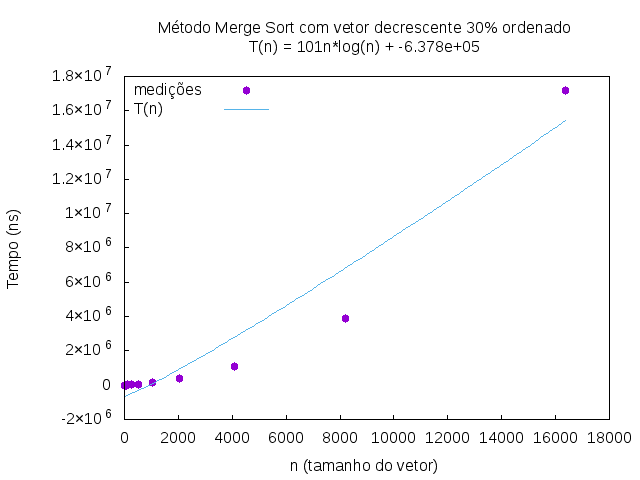
\includegraphics[width=0.7\linewidth]{graficos/MergeSort/vIntDecrescenteP30/vIntDecrescenteP30.png}
  \caption{Gráfico Merge Sort - Vetor Decrescente P30}
\end{figure}

\section{Merge Sort - Vetor Decrescente P40}
Tabela gerada utilizando Merge Sort com vetores de tamanho n, sendo n = $(2^k)$, de k = 4..14 e inseridos em ordem decrescente estando 40\% ordenado.
\begin{table}[H]
\centering
\caption{Merge Sort com vetor ordenado em ordem decrescente estando 40\% ordenado}
\label{my-label}
\begin{tabular}{|l|l|}
\hline
\multicolumn{1}{|c|}{\textbf{Número de Elementos}} & \multicolumn{1}{c|}{\textbf{Tempo de execução em nanosegundos}} \\ \hline
16 & 2161 \\ \hline
32 & 3295 \\ \hline
64 & 6402 \\ \hline
128 & 13101 \\ \hline
256 & 27715 \\ \hline
512 & 62184 \\ \hline
1024 & 147490 \\ \hline
2048 & 367866 \\ \hline
4096 & 1080496 \\ \hline
8192 & 3878299 \\ \hline
16384 & 17404245 \\ \hline
\end{tabular}
\end{table}

\subsection{Gráfico Merge Sort - Vetor Decrescente P40}
\begin{figure}[H]
    \centering
    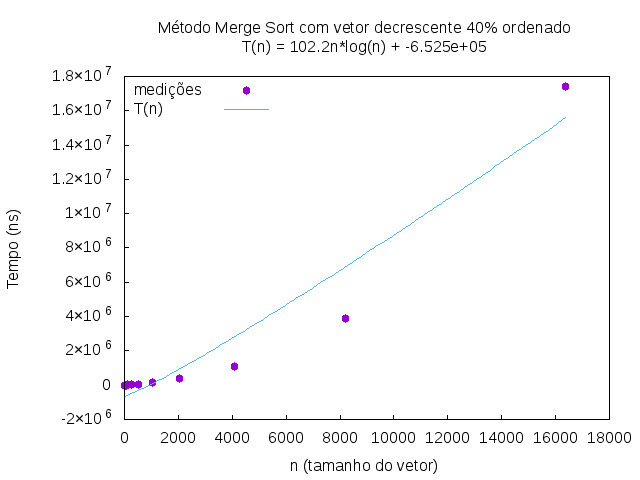
\includegraphics[width=0.7\linewidth]{graficos/MergeSort/vIntDecrescenteP40/vIntDecrescenteP40.png}
  \caption{Gráfico Merge Sort - Vetor Decrescente P40}
\end{figure}

\section{Merge Sort - Vetor Decrescente P50}
Tabela gerada utilizando Merge Sort com vetores de tamanho n, sendo n = $(2^k)$, de k = 4..14 e inseridos em ordem decrescente estando 50\% ordenado.
\begin{table}[H]
\centering
\caption{Merge Sort com vetor ordenado em ordem decrescente estando 50\% ordenado}
\label{my-label}
\begin{tabular}{|l|l|}
\hline
\multicolumn{1}{|c|}{\textbf{Número de Elementos}} & \multicolumn{1}{c|}{\textbf{Tempo de execução em nanosegundos}} \\ \hline
16 & 2166 \\ \hline
32 & 3258 \\ \hline
64 & 6530 \\ \hline
128 & 12686 \\ \hline
256 & 28095 \\ \hline
512 & 65430 \\ \hline
1024 & 151006 \\ \hline
2048 & 365972 \\ \hline
4096 & 1070690 \\ \hline
8192 & 3858348 \\ \hline
16384 & 17428128 \\ \hline
\end{tabular}
\end{table}

\subsection{Gráfico Merge Sort - Vetor Decrescente P50}
\begin{figure}[H]
    \centering
    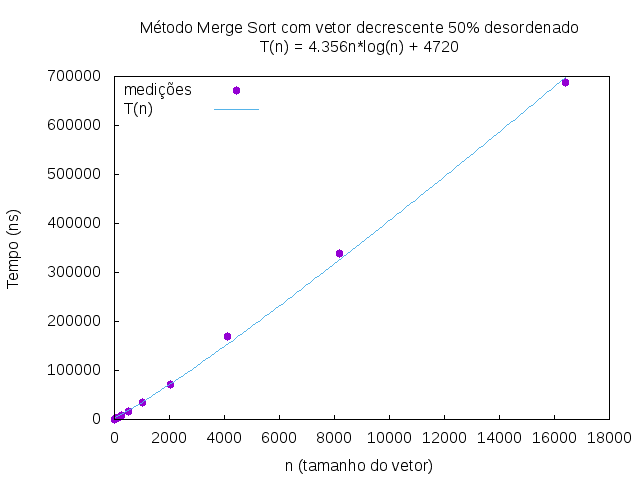
\includegraphics[width=0.7\linewidth]{graficos/MergeSort/vIntDecrescenteP50/vIntDecrescenteP50.png}
  \caption{Gráfico Merge Sort - Vetor Decrescente P50}
\end{figure}
\section{Observações Finais}
Merge sort com vetor de elementos totalmente aleatório levaria aproximadamente 2 horas e 49 minutos para processar um vetor de $2^k$ com k = 32 elementos nessas condições.

\chapter{Heap Sort}
O algoritmo de ordenação Heap Sort é um algoritmo não estável. Ele faz uso de uma estrutura chamadas heap e ordena os elementos a medida que insere na estrutura, assim ao terminar as inserções, os elementos podem ser removidos da raíz sucessivamente na ordem desejada, mantendo a propriedade de max-heap(ou min-heap).
Ele basicamente funciona montando uma árvore binária.
Em qualquer caso, temos que o algoritmo HeapSort tem complexidade de tempo $\theta(nlogn)$.

\section{Heap Sort - Vetor Aleatório}
Tabela gerada utilizando Heap Sort com vetores de tamanho n, sendo n = $(2^k)$, de k = 4..14 e inseridos aleatóriamente.
\begin{table}[H]
\centering
\caption{Heap Sort com vetor aleatório}
\label{my-label}
\begin{tabular}{|l|l|}
\hline
\multicolumn{1}{|c|}{\textbf{Número de Elementos}} & \multicolumn{1}{c|}{\textbf{Tempo de execução em nanosegundos}} \\ \hline
16 & 725 \\ \hline
32 & 971 \\ \hline
64 & 2123 \\ \hline
128 & 5011 \\ \hline
256 & 10633 \\ \hline
512 & 27914 \\ \hline
1024 & 65078 \\ \hline
2048 & 145462 \\ \hline
4096 & 318047 \\ \hline
8192 & 697040 \\ \hline
16384 & 1635985 \\ \hline
\end{tabular}
\end{table}

\subsection{Gráfico Heap Sort - Vetor Aleatório}
\begin{figure}[H]
    \centering
    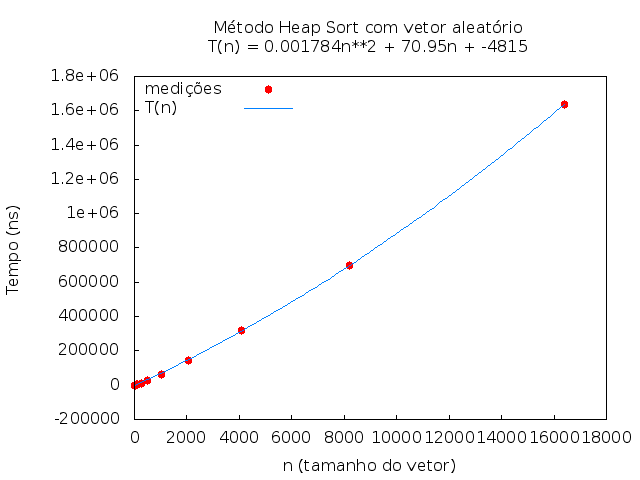
\includegraphics[width=0.7\linewidth]{graficos/HeapSort/vIntAleatorio/vIntAleatorio.png}
  \caption{Gráfico Heap Sort - Vetor Aleatório}
\end{figure}

\section{Heap Sort - Vetor Crescente}
Tabela gerada utilizando Heap Sort com vetores de tamanho n, sendo n = $(2^k)$, de k = 4..14 e inseridos em ordem crescente.
\begin{table}[H]
\centering
\caption{Heap Sort com vetor ordenado em ordem crescente}
\label{my-label}
\begin{tabular}{|l|l|}
\hline
\multicolumn{1}{|c|}{\textbf{Número de Elementos}} & \multicolumn{1}{c|}{\textbf{Tempo de execução em nanosegundos}} \\ \hline
16 & 842 \\ \hline
32 & 1075 \\ \hline
64 & 1668 \\ \hline
128 & 9925 \\ \hline
256 & 10534 \\ \hline
512 & 26131 \\ \hline
1024 & 57088 \\ \hline
2048 & 124606 \\ \hline
4096 & 218104 \\ \hline
8192 & 499002 \\ \hline
16384 & 959418 \\ \hline
\end{tabular}
\end{table}

\subsection{Gráfico Heap Sort - Vetor Crescente}
\begin{figure}[H]
    \centering
    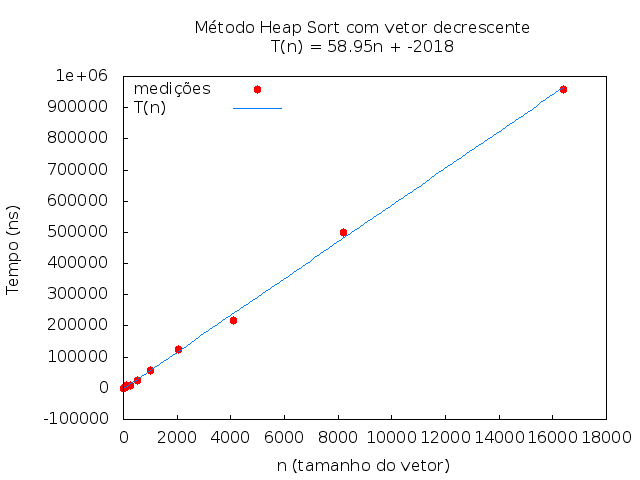
\includegraphics[width=0.7\linewidth]{graficos/HeapSort/vIntCrescente/vIntCrescente.png}
  \caption{Gráfico Heap Sort - Vetor Crescente}
\end{figure}

\section{Heap Sort - Vetor Crescente P10}
Tabela gerada utilizando Heap Sort com vetores de tamanho n, sendo n = $(2^k)$, de k = 4..14 e inseridos em ordem crescente estando 10\% ordenado.
\begin{table}[H]
\centering
\caption{Heap Sort com vetor ordenado em ordem crescente estando 10\% ordenado}
\label{my-label}
\begin{tabular}{|l|l|}
\hline
\multicolumn{1}{|c|}{\textbf{Número de Elementos}} & \multicolumn{1}{c|}{\textbf{Tempo de execução em nanosegundos}} \\ \hline
16 & 573 \\ \hline
32 & 792 \\ \hline
64 & 1669 \\ \hline
128 & 3719 \\ \hline
256 & 9700 \\ \hline
512 & 25058 \\ \hline
1024 & 55952 \\ \hline
2048 & 121179 \\ \hline
4096 & 238053 \\ \hline
8192 & 451335 \\ \hline
16384 & 946165 \\ \hline
\end{tabular}
\end{table}

\subsection{Gráfico Heap Sort - Vetor Crescente P10}
\begin{figure}[H]
    \centering
    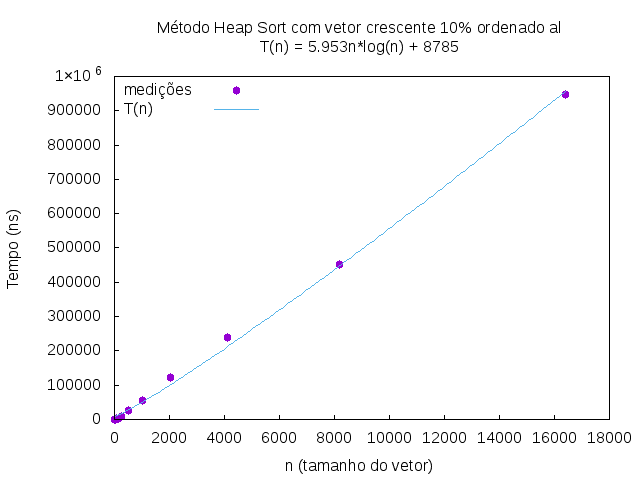
\includegraphics[width=0.7\linewidth]{graficos/HeapSort/vIntCrescenteP10/vIntCrescenteP10.png}
  \caption{Gráfico Heap Sort - Vetor Crescente P10}
\end{figure}

\section{Heap Sort - Vetor Crescente P20}
Tabela gerada utilizando Heap Sort com vetores de tamanho n, sendo n = $(2^k)$, de k = 4..14 e inseridos em ordem crescente estando 20\% ordenado.
\begin{table}[H]
\centering
\caption{Heap Sort com vetor ordenado em ordem crescente estando 20\% ordenado}
\label{my-label}
\begin{tabular}{|l|l|}
\hline
\multicolumn{1}{|c|}{\textbf{Número de Elementos}} & \multicolumn{1}{c|}{\textbf{Tempo de execução em nanosegundos}} \\ \hline
16 & 534 \\ \hline
32 & 875 \\ \hline
64 & 1628 \\ \hline
128 & 4073 \\ \hline
256 & 9612 \\ \hline
512 & 25183 \\ \hline
1024 & 60872 \\ \hline
2048 & 127670 \\ \hline
4096 & 228395 \\ \hline
8192 & 472599 \\ \hline
16384 & 957241 \\ \hline
\end{tabular}
\end{table}

\subsection{Gráfico Heap Sort - Vetor Crescente P20}
\begin{figure}[H]
    \centering
    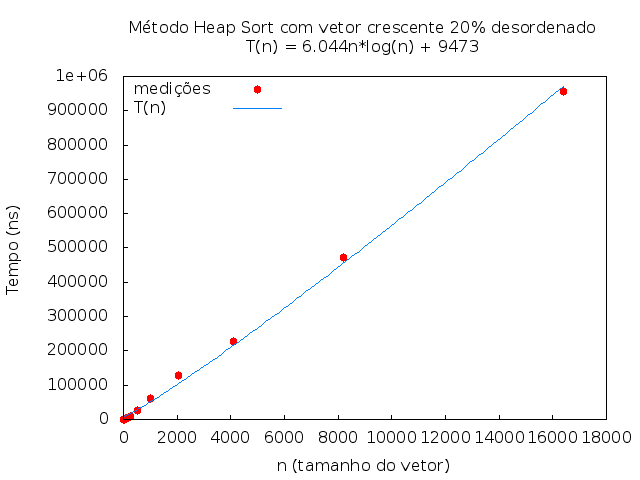
\includegraphics[width=0.7\linewidth]{graficos/HeapSort/vIntCrescenteP20/vIntCrescenteP20.png}
  \caption{Gráfico Heap Sort - Vetor Crescente P20}
\end{figure}

\section{Heap Sort - Vetor Crescente P30}
Tabela gerada utilizando Heap Sort com vetores de tamanho n, sendo n = $(2^k)$, de k = 4..14 e inseridos em ordem crescente estando 30\% ordenado.
\begin{table}[H]
\centering
\caption{Heap Sort com vetor ordenado em ordem crescente estando 30\% ordenado}
\label{my-label}
\begin{tabular}{|l|l|}
\hline
\multicolumn{1}{|c|}{\textbf{Número de Elementos}} & \multicolumn{1}{c|}{\textbf{Tempo de execução em nanosegundos}} \\ \hline
16 & 510 \\ \hline
32 & 862 \\ \hline
64 & 1630 \\ \hline
128 & 3750 \\ \hline
256 & 9836 \\ \hline
512 & 24383 \\ \hline
1024 & 65255 \\ \hline
2048 & 122553 \\ \hline
4096 & 241699 \\ \hline
8192 & 493026 \\ \hline
16384 & 954964 \\ \hline
\end{tabular}
\end{table}

\subsection{Gráfico Heap Sort - Vetor Crescente P30}
\begin{figure}[H]
    \centering
    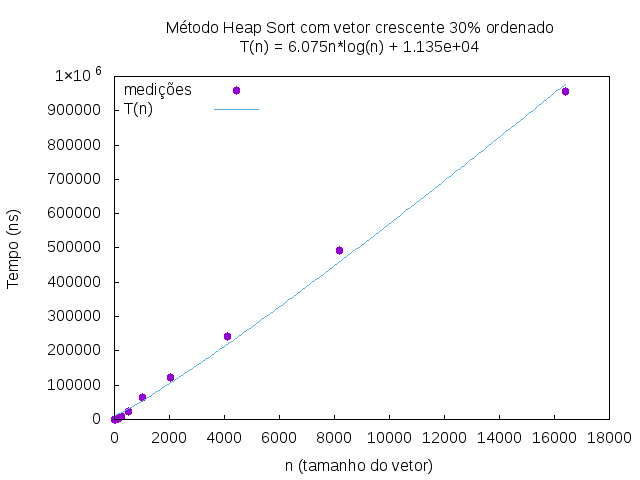
\includegraphics[width=0.7\linewidth]{graficos/HeapSort/vIntCrescenteP30/vIntCrescenteP30.png}
  \caption{Gráfico Heap Sort - Vetor Crescente P30}
\end{figure}

\section{Heap Sort - Vetor Crescente P40}
Tabela gerada utilizando Heap Sort com vetores de tamanho n, sendo n = $(2^k)$, de k = 4..14 e inseridos em ordem crescente estando 40\% ordenado.
\begin{table}[H]
\centering
\caption{Heap Sort com vetor ordenado em ordem crescente estando 40\% ordenado}
\label{my-label}
\begin{tabular}{|l|l|}
\hline
\multicolumn{1}{|c|}{\textbf{Número de Elementos}} & \multicolumn{1}{c|}{\textbf{Tempo de execução em nanosegundos}} \\ \hline
16 & 501 \\ \hline
32 & 786 \\ \hline
64 & 1799 \\ \hline
128 & 9422 \\ \hline
256 & 10202 \\ \hline
512 & 25220 \\ \hline
1024 & 55734 \\ \hline
2048 & 112945 \\ \hline
4096 & 233312 \\ \hline
8192 & 479594 \\ \hline
16384 & 947705 \\ \hline
\end{tabular}
\end{table}

\subsection{Gráfico Heap Sort - Vetor Crescente P40}
\begin{figure}[H]
    \centering
    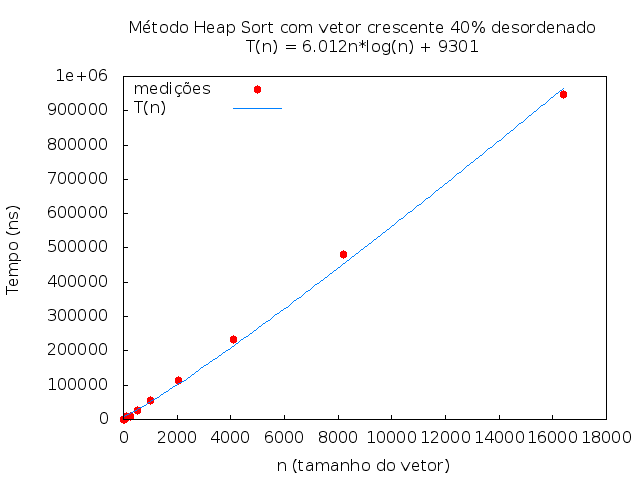
\includegraphics[width=0.7\linewidth]{graficos/HeapSort/vIntCrescenteP40/vIntCrescenteP40.png}
  \caption{Gráfico Heap Sort - Vetor Crescente P40}
\end{figure}

\section{Heap Sort - Vetor Crescente P50}
Tabela gerada utilizando Heap Sort com vetores de tamanho n, sendo n = $(2^k)$, de k = 4..14 e inseridos em ordem crescente estando 50\% ordenado.
\begin{table}[H]
\centering
\caption{Heap Sort com vetor ordenado em ordem crescente estando 50\% ordenado}
\label{my-label}
\begin{tabular}{|l|l|}
\hline
\multicolumn{1}{|c|}{\textbf{Número de Elementos}} & \multicolumn{1}{c|}{\textbf{Tempo de execução em nanosegundos}} \\ \hline
16 & 546 \\ \hline
32 & 782 \\ \hline
64 & 1652 \\ \hline
128 & 3627 \\ \hline
256 & 16960 \\ \hline
512 & 27534 \\ \hline
1024 & 67128 \\ \hline
2048 & 114637 \\ \hline
4096 & 266050 \\ \hline
8192 & 477692 \\ \hline
16384 & 960498 \\ \hline
\end{tabular}
\end{table}

\subsection{Gráfico Heap Sort - Vetor Crescente P50}
\begin{figure}[H]
    \centering
    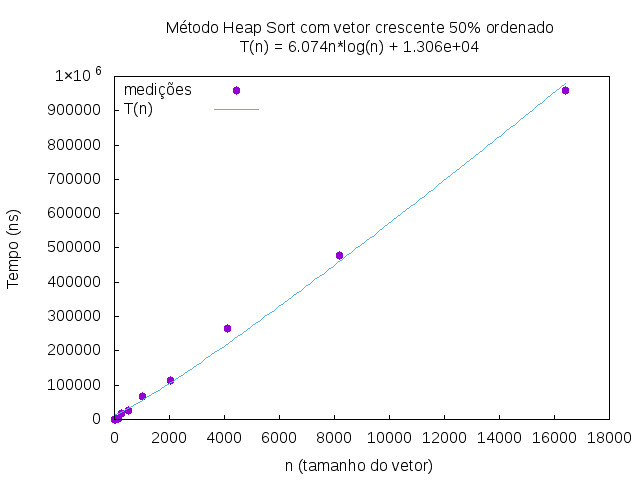
\includegraphics[width=0.7\linewidth]{graficos/HeapSort/vIntCrescenteP50/vIntCrescenteP50.png}
  \caption{Gráfico Heap Sort - Vetor Crescente P50}
\end{figure}

\section{Heap Sort - Vetor Decrescente}
Tabela gerada utilizando Heap Sort com vetores de tamanho n, sendo n = $(2^k)$, de k = 4..14 e inseridos em ordem decrescente.
\begin{table}[H]
\centering
\caption{Heap Sort com vetor ordenado em ordem decrescente}
\label{my-label}
\begin{tabular}{|l|l|}
\hline
\multicolumn{1}{|c|}{\textbf{Número de Elementos}} & \multicolumn{1}{c|}{\textbf{Tempo de execução em nanosegundos}} \\ \hline
16 & 497 \\ \hline
32 & 723 \\ \hline
64 & 1485 \\ \hline
128 & 3515 \\ \hline
256 & 9684 \\ \hline
512 & 23405 \\ \hline
1024 & 55215 \\ \hline
2048 & 121471 \\ \hline
4096 & 238966 \\ \hline
8192 & 492005 \\ \hline
16384 & 1021937 \\ \hline
\end{tabular}
\end{table}

\subsection{Gráfico Heap Sort - Vetor Decrescente}
\begin{figure}[H]
    \centering
    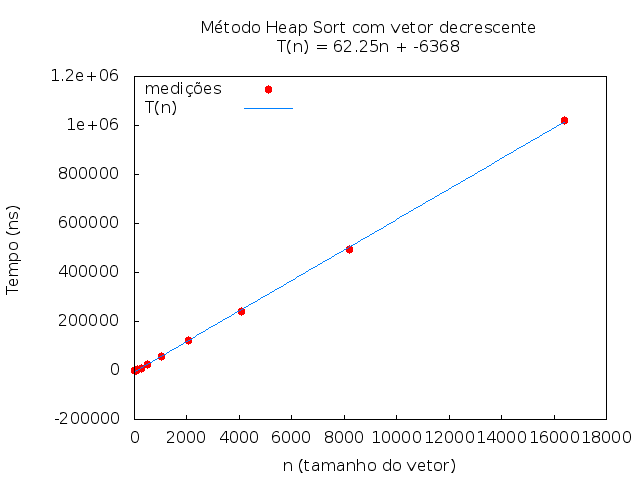
\includegraphics[width=0.7\linewidth]{graficos/HeapSort/vIntDecrescente/vIntDecrescente.png}
  \caption{Gráfico Heap Sort - Vetor Decrescente}
\end{figure}

\section{Heap Sort - Vetor Decrescente P10}
Tabela gerada utilizando Heap Sort com vetores de tamanho n, sendo n = $(2^k)$, de k = 4..14 e inseridos em ordem decrescente estando 10\% ordenado.
\begin{table}[H]
\centering
\caption{Heap Sort com vetor ordenado em ordem decrescente estando 10\% ordenado}
\label{my-label}
\begin{tabular}{|l|l|}
\hline
\multicolumn{1}{|c|}{\textbf{Número de Elementos}} & \multicolumn{1}{c|}{\textbf{Tempo de execução em nanosegundos}} \\ \hline
16 & 533 \\ \hline
32 & 885 \\ \hline
64 & 1825 \\ \hline
128 & 3787 \\ \hline
256 & 9940 \\ \hline
512 & 24112 \\ \hline
1024 & 55700 \\ \hline
2048 & 131589 \\ \hline
4096 & 239256 \\ \hline
8192 & 497985 \\ \hline
16384 & 1019311 \\ \hline
\end{tabular}
\end{table}

\subsection{Gráfico Heap Sort - Vetor Decrescente P10}
\begin{figure}[H]
    \centering
    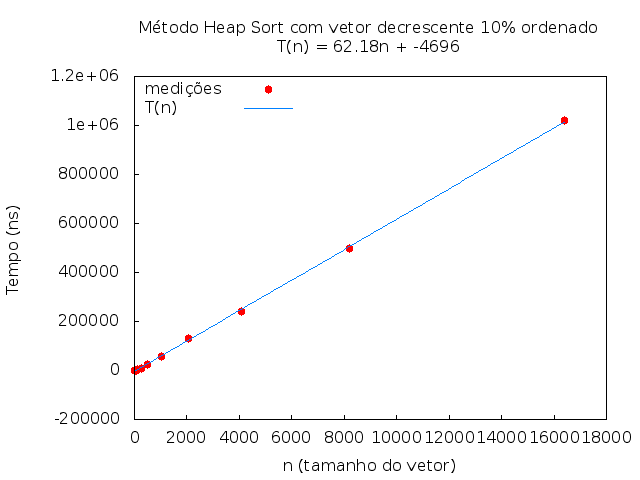
\includegraphics[width=0.7\linewidth]{graficos/HeapSort/vIntDecrescenteP10/vIntDecrescenteP10.png}
  \caption{Gráfico Heap Sort - Vetor Decrescente P10}
\end{figure}

\section{Heap Sort - Vetor Decrescente P20}
Tabela gerada utilizando Heap Sort com vetores de tamanho n, sendo n = $(2^k)$, de k = 4..14 e inseridos em ordem decrescente estando 20\% ordenado.
\begin{table}[H]
\centering
\caption{Heap Sort com vetor ordenado em ordem decrescente estando 20\% ordenado}
\label{my-label}
\begin{tabular}{|l|l|}
\hline
\multicolumn{1}{|c|}{\textbf{Número de Elementos}} & \multicolumn{1}{c|}{\textbf{Tempo de execução em nanosegundos}} \\ \hline
16 & 552 \\ \hline
32 & 851 \\ \hline
64 & 1775 \\ \hline
128 & 4138 \\ \hline
256 & 10415 \\ \hline
512 & 34619 \\ \hline
1024 & 56092 \\ \hline
2048 & 120560 \\ \hline
4096 & 236652 \\ \hline
8192 & 505112 \\ \hline
16384 & 991519 \\ \hline
\end{tabular}
\end{table}

\subsection{Gráfico Heap Sort - Vetor Decrescente P20}
\begin{figure}[H]
    \centering
    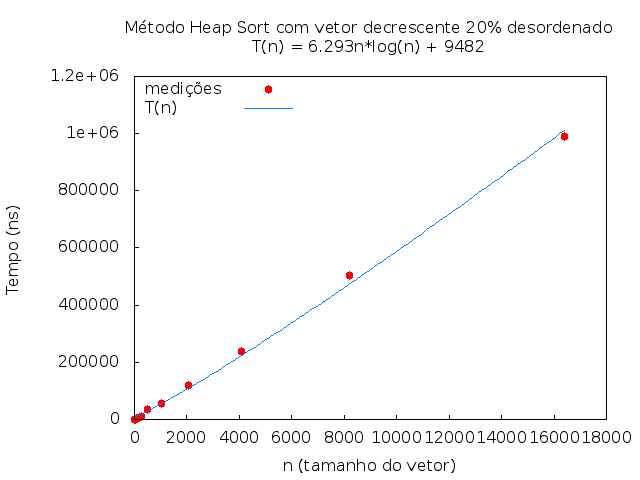
\includegraphics[width=0.7\linewidth]{graficos/HeapSort/vIntDecrescenteP20/vIntDecrescenteP20.png}
  \caption{Gráfico Heap Sort - Vetor Decrescente P20}
\end{figure}

\section{Heap Sort - Vetor Decrescente P30}
Tabela gerada utilizando Heap Sort com vetores de tamanho n, sendo n = $(2^k)$, de k = 4..14 e inseridos em ordem decrescente estando 30\% ordenado.
\begin{table}[H]
\centering
\caption{Heap Sort com vetor ordenado em ordem decrescente estando 30\% ordenado}
\label{my-label}
\begin{tabular}{|l|l|}
\hline
\multicolumn{1}{|c|}{\textbf{Número de Elementos}} & \multicolumn{1}{c|}{\textbf{Tempo de execução em nanosegundos}} \\ \hline
16 & 574 \\ \hline
32 & 901 \\ \hline
64 & 1805 \\ \hline
128 & 4445 \\ \hline
256 & 9851 \\ \hline
512 & 25314 \\ \hline
1024 & 58946 \\ \hline
2048 & 115970 \\ \hline
4096 & 236945 \\ \hline
8192 & 517471 \\ \hline
16384 & 1013956 \\ \hline
\end{tabular}
\end{table}

\subsection{Gráfico Heap Sort - Vetor Decrescente P30}
\begin{figure}[H]
    \centering
    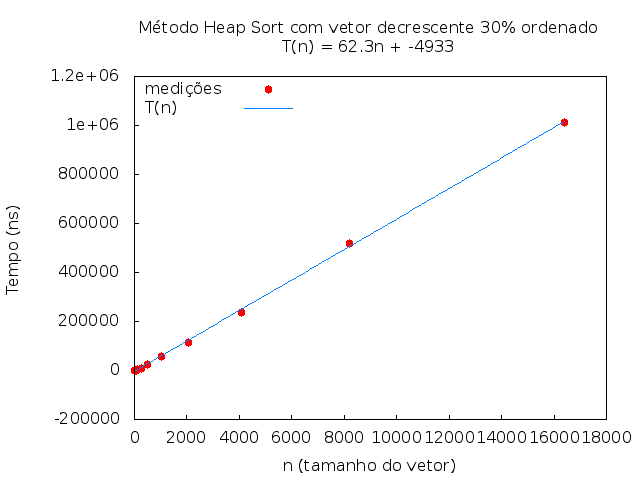
\includegraphics[width=0.7\linewidth]{graficos/HeapSort/vIntDecrescenteP30/vIntDecrescenteP30.png}
  \caption{Gráfico Heap Sort - Vetor Decrescente P30}
\end{figure}

\section{Heap Sort - Vetor Decrescente P40}
Tabela gerada utilizando Heap Sort com vetores de tamanho n, sendo n = $(2^k)$, de k = 4..14 e inseridos em ordem decrescente estando 40\% ordenado.
\begin{table}[H]
\centering
\caption{Heap Sort com vetor ordenado em ordem decrescente estando 40\% ordenado}
\label{my-label}
\begin{tabular}{|l|l|}
\hline
\multicolumn{1}{|c|}{\textbf{Número de Elementos}} & \multicolumn{1}{c|}{\textbf{Tempo de execução em nanosegundos}} \\ \hline
16 & 566 \\ \hline
32 & 878 \\ \hline
64 & 1773 \\ \hline
128 & 3932 \\ \hline
256 & 9781 \\ \hline
512 & 24638 \\ \hline
1024 & 55357 \\ \hline
2048 & 117612 \\ \hline
4096 & 247034 \\ \hline
8192 & 479714 \\ \hline
16384 & 966254 \\ \hline
\end{tabular}
\end{table}

\subsection{Gráfico Heap Sort - Vetor Decrescente P40}
\begin{figure}[H]
    \centering
    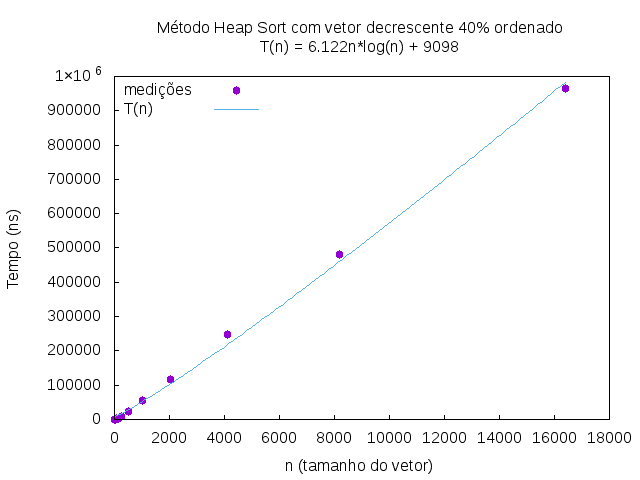
\includegraphics[width=0.7\linewidth]{graficos/HeapSort/vIntDecrescenteP40/vIntDecrescenteP40.png}
  \caption{Gráfico Heap Sort - Vetor Decrescente P40}
\end{figure}

\section{Heap Sort - Vetor Decrescente P50}
Tabela gerada utilizando Heap Sort com vetores de tamanho n, sendo n = $(2^k)$, de k = 4..14 e inseridos em ordem decrescente estando 50\% ordenado.
\begin{table}[H]
\centering
\caption{Heap Sort com vetor ordenado em ordem decrescente estando 50\% ordenado}
\label{my-label}
\begin{tabular}{|l|l|}
\hline
\multicolumn{1}{|c|}{\textbf{Número de Elementos}} & \multicolumn{1}{c|}{\textbf{Tempo de execução em nanosegundos}} \\ \hline
16 & 676 \\ \hline
32 & 949 \\ \hline
64 & 1959 \\ \hline
128 & 4289 \\ \hline
256 & 10597 \\ \hline
512 & 24941 \\ \hline
1024 & 54696 \\ \hline
2048 & 138827 \\ \hline
4096 & 236799 \\ \hline
8192 & 531128 \\ \hline
16384 & 947050 \\ \hline
\end{tabular}
\end{table}

\subsection{Gráfico Heap Sort - Vetor Decrescente P50}
\begin{figure}[H]
    \centering
    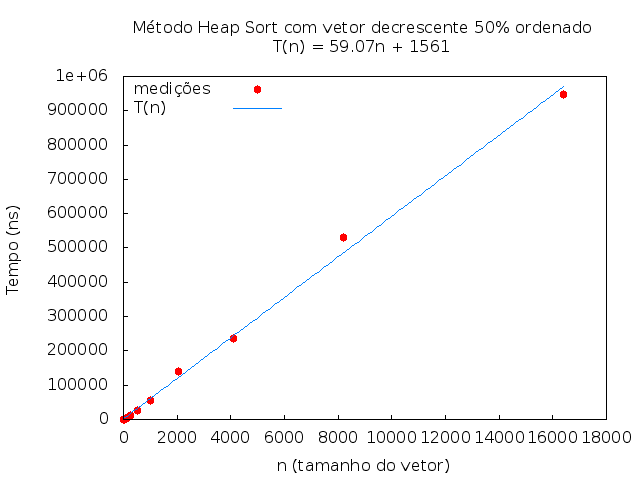
\includegraphics[width=0.7\linewidth]{graficos/HeapSort/vIntDecrescenteP50/vIntDecrescenteP50.png}
  \caption{Gráfico Heap Sort - Vetor Decrescente P50}
\end{figure}
\section{Observações Finais}
heap sort com vetor em ordem decrescente com 10\% dos elementos ordenados levaria aproximadamente 10 minutos para processar um vetor de $2^k$ com k = 32 elementos.

\chapter{Quick Sort}
QuickSort adota a estratégia de divisão e conquista, basicamente ele trabalha escolhendo um pivo, ele rearranja a lista da forma que os maiores que pivo ficam a direita e menores a esquerda, ele faz isso recursivamente até que tenha uma lista ordenada.
Em qualquer caso, temos que o algoritmo QuickSort tem complexidade de tempo O$(n^2)$ no pior caso e tanto no médio quanto no melhor caso é O(nlogn).

\section{Quick Sort - Vetor Aleatório}
Tabela gerada utilizando Quick Sort com vetores de tamanho n, sendo n = $(2^k)$, de k = 4..14 e inseridos aleatóriamente.
\begin{table}[H]
\centering
\caption{Quick Sort com vetor aleatório}
\label{my-label}
\begin{tabular}{|l|l|}
\hline
\multicolumn{1}{|c|}{\textbf{Número de Elementos}} & \multicolumn{1}{c|}{\textbf{Tempo de execução em nanosegundos}} \\ \hline
16 & 925 \\ \hline
32 & 1077 \\ \hline
64 & 2100 \\ \hline
128 & 4491 \\ \hline
256 & 10525 \\ \hline
512 & 23829 \\ \hline
1024 & 62993 \\ \hline
2048 & 125500 \\ \hline
4096 & 278666 \\ \hline
8192 & 576399 \\ \hline
16384 & 1261602 \\ \hline
\end{tabular}
\end{table}

\subsection{Gráfico Quick Sort - Vetor Aleatório}
\begin{figure}[H]
    \centering
    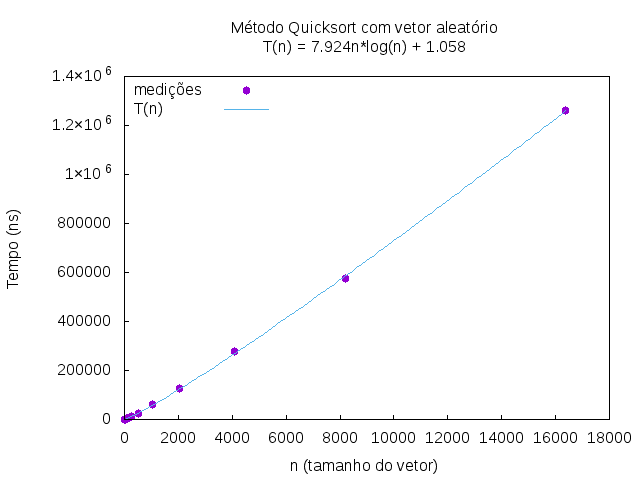
\includegraphics[width=0.7\linewidth]{graficos/QuickSort/vIntAleatorio/vIntAleatorio.png}
  \caption{Gráfico Quick Sort - Vetor Aleatório}
\end{figure}

\section{Quick Sort - Vetor Crescente}
Tabela gerada utilizando Quick Sort com vetores de tamanho n, sendo n = $(2^k)$, de k = 4..14 e inseridos em ordem crescente.
\begin{table}[H]
\centering
\caption{Quick Sort com vetor ordenado em ordem crescente}
\label{my-label}
\begin{tabular}{|l|l|}
\hline
\multicolumn{1}{|c|}{\textbf{Número de Elementos}} & \multicolumn{1}{c|}{\textbf{Tempo de execução em nanosegundos}} \\ \hline
16 & 706 \\ \hline
32 & 954 \\ \hline
64 & 1363 \\ \hline
128 & 2163 \\ \hline
256 & 3711 \\ \hline
512 & 7086 \\ \hline
1024 & 13945 \\ \hline
2048 & 28288 \\ \hline
4096 & 61831 \\ \hline
8192 & 127886 \\ \hline
16384 & 299130 \\ \hline
\end{tabular}
\end{table}

\subsection{Gráfico Quick Sort - Vetor Crescente}
\begin{figure}[H]
    \centering
    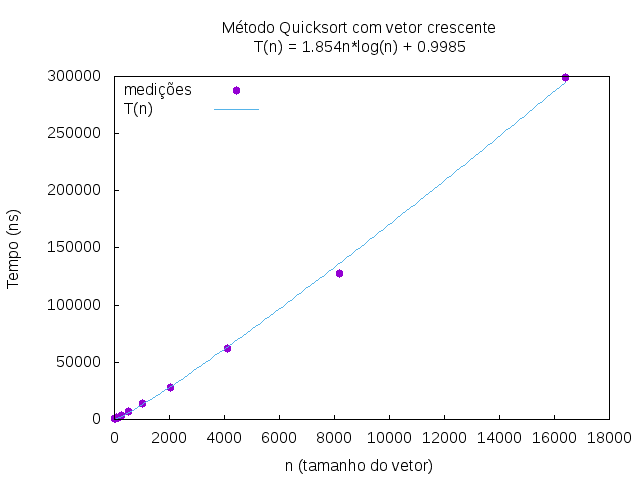
\includegraphics[width=0.7\linewidth]{graficos/QuickSort/vIntCrescente/vIntCrescente.png}
  \caption{Gráfico Quick Sort - Vetor Crescente}
\end{figure}

\section{Quick Sort - Vetor Crescente P10}
Tabela gerada utilizando Quick Sort com vetores de tamanho n, sendo n = $(2^k)$, de k = 4..14 e inseridos em ordem crescente estando 10\% ordenado.
\begin{table}[H]
\centering
\caption{Quick Sort com vetor ordenado em ordem crescente estando 10\% ordenado}
\label{my-label}
\begin{tabular}{|l|l|}
\hline
\multicolumn{1}{|c|}{\textbf{Número de Elementos}} & \multicolumn{1}{c|}{\textbf{Tempo de execução em nanosegundos}} \\ \hline
16 & 574 \\ \hline
32 & 829 \\ \hline
64 & 1158 \\ \hline
128 & 2138 \\ \hline
256 & 3617 \\ \hline
512 & 6888 \\ \hline
1024 & 13829 \\ \hline
2048 & 28293 \\ \hline
4096 & 60946 \\ \hline
8192 & 131339 \\ \hline
16384 & 269900 \\ \hline
\end{tabular}
\end{table}

\subsection{Gráfico Quick Sort - Vetor Crescente P10}
\begin{figure}[H]
    \centering
    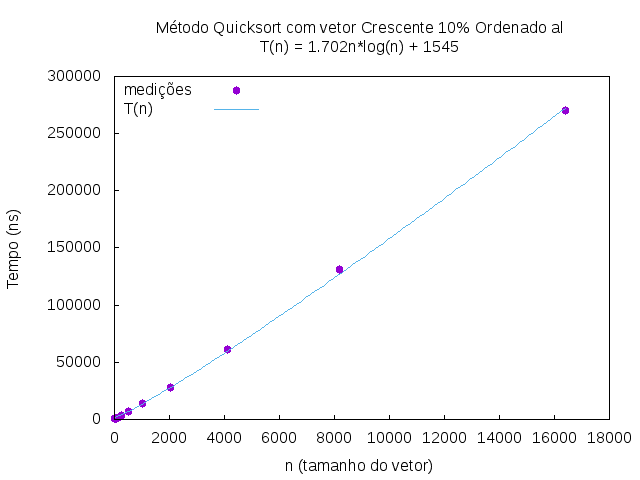
\includegraphics[width=0.7\linewidth]{graficos/QuickSort/vIntCrescenteP10/vIntCrescenteP10.png}
  \caption{Gráfico Quick Sort - Vetor Crescente P10}
\end{figure}

\section{Quick Sort - Vetor Crescente P20}
Tabela gerada utilizando Quick Sort com vetores de tamanho n, sendo n = $(2^k)$, de k = 4..14 e inseridos em ordem crescente estando 20\% ordenado.
\begin{table}[H]
\centering
\caption{Quick Sort com vetor ordenado em ordem crescente estando 20\% ordenado}
\label{my-label}
\begin{tabular}{|l|l|}
\hline
\multicolumn{1}{|c|}{\textbf{Número de Elementos}} & \multicolumn{1}{c|}{\textbf{Tempo de execução em nanosegundos}} \\ \hline
16 & 685 \\ \hline
32 & 807 \\ \hline
64 & 1334 \\ \hline
128 & 2136 \\ \hline
256 & 3568 \\ \hline
512 & 6805 \\ \hline
1024 & 13583 \\ \hline
2048 & 27666 \\ \hline
4096 & 56503 \\ \hline
8192 & 121141 \\ \hline
16384 & 264576 \\ \hline
\end{tabular}
\end{table}

\subsection{Gráfico Quick Sort - Vetor Crescente P20}
\begin{figure}[H]
    \centering
    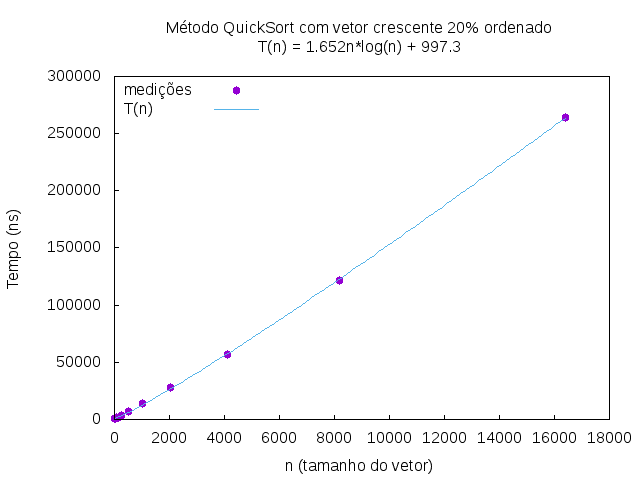
\includegraphics[width=0.7\linewidth]{graficos/QuickSort/vIntCrescenteP20/vIntCrescenteP20.png}
  \caption{Gráfico Quick Sort - Vetor Crescente P20}
\end{figure}

\section{Quick Sort - Vetor Crescente P30}
Tabela gerada utilizando Quick Sort com vetores de tamanho n, sendo n = $(2^k)$, de k = 4..14 e inseridos em ordem crescente estando 30\% ordenado.
\begin{table}[H]
\centering
\caption{Quick Sort com vetor ordenado em ordem crescente estando 30\% ordenado}
\label{my-label}
\begin{tabular}{|l|l|}
\hline
\multicolumn{1}{|c|}{\textbf{Número de Elementos}} & \multicolumn{1}{c|}{\textbf{Tempo de execução em nanosegundos}} \\ \hline
16 & 651 \\ \hline
32 & 919 \\ \hline
64 & 1282 \\ \hline
128 & 2141 \\ \hline
256 & 3705 \\ \hline
512 & 6656 \\ \hline
1024 & 13097 \\ \hline
2048 & 27936 \\ \hline
4096 & 66555 \\ \hline
8192 & 121364 \\ \hline
16384 & 248146 \\ \hline
\end{tabular}
\end{table}

\subsection{Gráfico Quick Sort - Vetor Crescente P30}
\begin{figure}[H]
    \centering
    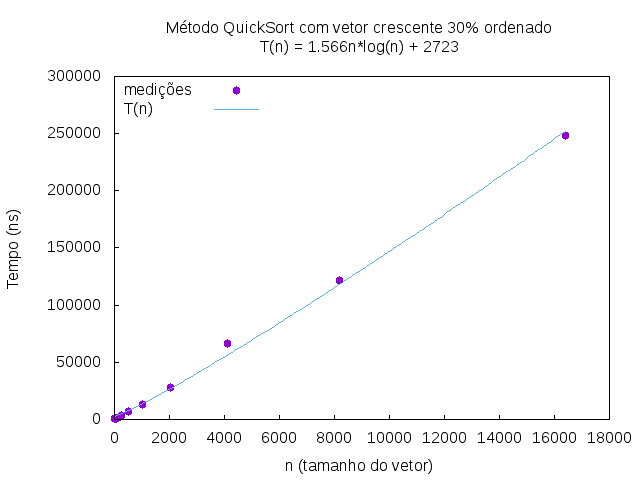
\includegraphics[width=0.7\linewidth]{graficos/QuickSort/vIntCrescenteP30/vIntCrescenteP30.png}
  \caption{Gráfico Quick Sort - Vetor Crescente P30}
\end{figure}

\section{Quick Sort - Vetor Crescente P40}
Tabela gerada utilizando Quick Sort com vetores de tamanho n, sendo n = $(2^k)$, de k = 4..14 e inseridos em ordem crescente estando 40\% ordenado.
\begin{table}[H]
\centering
\caption{Quick Sort com vetor ordenado em ordem crescente estando 40\% ordenado}
\label{my-label}
\begin{tabular}{|l|l|}
\hline
\multicolumn{1}{|c|}{\textbf{Número de Elementos}} & \multicolumn{1}{c|}{\textbf{Tempo de execução em nanosegundos}} \\ \hline
16 & 549 \\ \hline
32 & 879 \\ \hline
64 & 1148 \\ \hline
128 & 1817 \\ \hline
256 & 3197 \\ \hline
512 & 6362 \\ \hline
1024 & 12558 \\ \hline
2048 & 31216 \\ \hline
4096 & 53019 \\ \hline
8192 & 120388 \\ \hline
16384 & 238560 \\ \hline
\end{tabular}
\end{table}

\subsection{Gráfico Quick Sort - Vetor Crescente P40}
\begin{figure}[H]
    \centering
    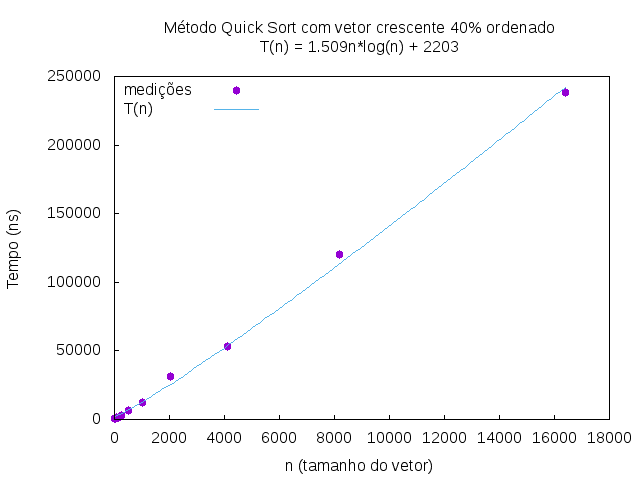
\includegraphics[width=0.7\linewidth]{graficos/QuickSort/vIntCrescenteP40/vIntCrescenteP40.png}
  \caption{Gráfico Quick Sort - Vetor Crescente P40}
\end{figure}

\section{Quick Sort - Vetor Crescente P50}
Tabela gerada utilizando Quick Sort com vetores de tamanho n, sendo n = $(2^k)$, de k = 4..14 e inseridos em ordem crescente estando 50\% ordenado.
\begin{table}[H]
\centering
\caption{Quick Sort com vetor ordenado em ordem crescente estando 50\% ordenado}
\label{my-label}
\begin{tabular}{|l|l|}
\hline
\multicolumn{1}{|c|}{\textbf{Número de Elementos}} & \multicolumn{1}{c|}{\textbf{Tempo de execução em nanosegundos}} \\ \hline
16 & 560 \\ \hline
32 & 718 \\ \hline
64 & 1083 \\ \hline
128 & 1784 \\ \hline
256 & 3276 \\ \hline
512 & 6081 \\ \hline
1024 & 12595 \\ \hline
2048 & 26004 \\ \hline
4096 & 54648 \\ \hline
8192 & 145564 \\ \hline
16384 & 241835 \\ \hline
\end{tabular}
\end{table}

\subsection{Gráfico Quick Sort - Vetor Crescente P50}
\begin{figure}[H]
    \centering
    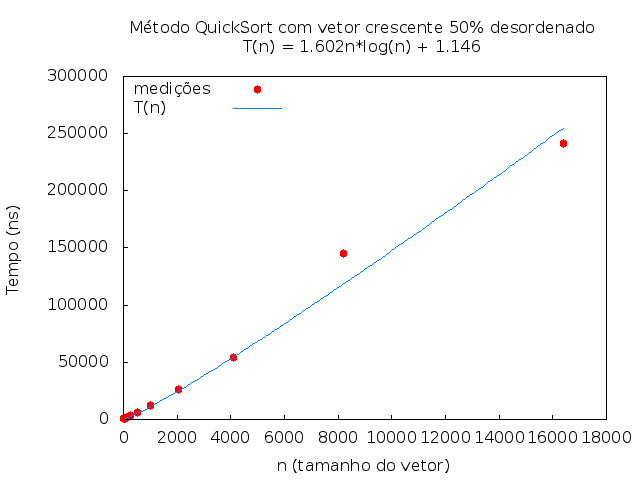
\includegraphics[width=0.7\linewidth]{graficos/QuickSort/vIntCrescenteP50/vIntCrescenteP50.png}
  \caption{Gráfico Quick Sort - Vetor Crescente P50}
\end{figure}

\section{Quick Sort - Vetor Decrescente}
Tabela gerada utilizando Quick Sort com vetores de tamanho n, sendo n = $(2^k)$, de k = 4..14 e inseridos em ordem decrescente.
\begin{table}[H]
\centering
\caption{Quick Sort com vetor ordenado em ordem decrescente}
\label{my-label}
\begin{tabular}{|l|l|}
\hline
\multicolumn{1}{|c|}{\textbf{Número de Elementos}} & \multicolumn{1}{c|}{\textbf{Tempo de execução em nanosegundos}} \\ \hline
16 & 589 \\ \hline
32 & 749 \\ \hline
64 & 883 \\ \hline
128 & 1476 \\ \hline
256 & 2584 \\ \hline
512 & 4991 \\ \hline
1024 & 9893 \\ \hline
2048 & 20693 \\ \hline
4096 & 50409 \\ \hline
8192 & 93702 \\ \hline
16384 & 201092 \\ \hline
\end{tabular}
\end{table}

\subsection{Gráfico Quick Sort - Vetor Decrescente}
\begin{figure}[H]
    \centering
    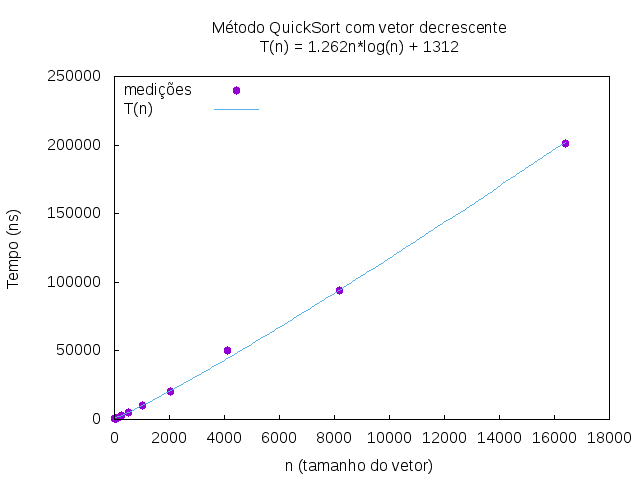
\includegraphics[width=0.7\linewidth]{graficos/QuickSort/vIntDecrescente/vIntDecrescente.png}
  \caption{Gráfico Quick Sort - Vetor Decrescente}
\end{figure}

\section{Quick Sort - Vetor Decrescente P10}
Tabela gerada utilizando Quick Sort com vetores de tamanho n, sendo n = $(2^k)$, de k = 4..14 e inseridos em ordem decrescente estando 10\% ordenado.
\begin{table}[H]
\centering
\caption{Quick Sort com vetor ordenado em ordem decrescente estando 10\% ordenado}
\label{my-label}
\begin{tabular}{|l|l|}
\hline
\multicolumn{1}{|c|}{\textbf{Número de Elementos}} & \multicolumn{1}{c|}{\textbf{Tempo de execução em nanosegundos}} \\ \hline
16 & 698 \\ \hline
32 & 701 \\ \hline
64 & 1162 \\ \hline
128 & 1805 \\ \hline
256 & 3019 \\ \hline
512 & 5849 \\ \hline
1024 & 11126 \\ \hline
2048 & 22521 \\ \hline
4096 & 49710 \\ \hline
8192 & 102070 \\ \hline
16384 & 222690 \\ \hline
\end{tabular}
\end{table}

\subsection{Gráfico Quick Sort - Vetor Decrescente P10}
\begin{figure}[H]
    \centering
    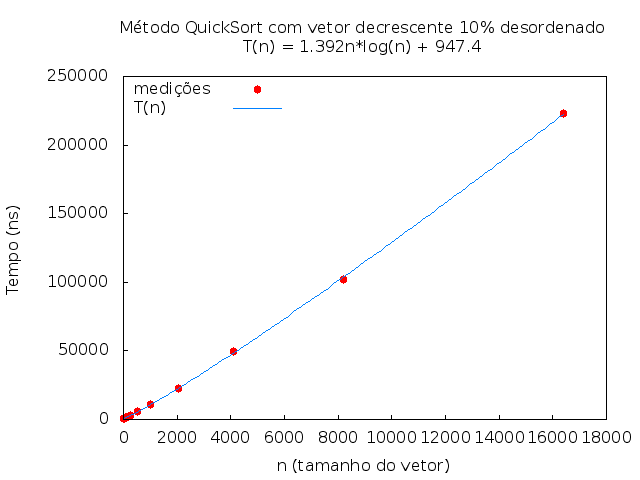
\includegraphics[width=0.7\linewidth]{graficos/QuickSort/vIntDecrescenteP10/vIntDecrescenteP10.png}
  \caption{Gráfico Quick Sort - Vetor Decrescente P10}
\end{figure}

\section{Quick Sort - Vetor Decrescente P20}
Tabela gerada utilizando Quick Sort com vetores de tamanho n, sendo n = $(2^k)$, de k = 4..14 e inseridos em ordem decrescente estando 20\% ordenado.
\begin{table}[H]
\centering
\caption{Quick Sort com vetor ordenado em ordem decrescente estando 20\% ordenado}
\label{my-label}
\begin{tabular}{|l|l|}
\hline
\multicolumn{1}{|c|}{\textbf{Número de Elementos}} & \multicolumn{1}{c|}{\textbf{Tempo de execução em nanosegundos}} \\ \hline
16 & 835 \\ \hline
32 & 868 \\ \hline
64 & 1218 \\ \hline
128 & 1905 \\ \hline
256 & 3398 \\ \hline
512 & 6020 \\ \hline
1024 & 11484 \\ \hline
2048 & 23470 \\ \hline
4096 & 48791 \\ \hline
8192 & 110327 \\ \hline
16384 & 218467 \\ \hline
\end{tabular}
\end{table}

\subsection{Gráfico Quick Sort - Vetor Decrescente P20}
\begin{figure}[H]
    \centering
    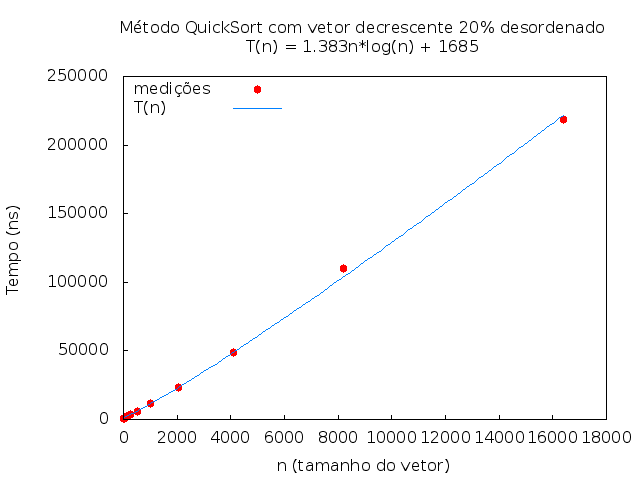
\includegraphics[width=0.7\linewidth]{graficos/QuickSort/vIntDecrescenteP20/vIntDecrescenteP20.png}
  \caption{Gráfico Quick Sort - Vetor Decrescente P20}
\end{figure}

\section{Quick Sort - Vetor Decrescente P30}
Tabela gerada utilizando Quick Sort com vetores de tamanho n, sendo n = $(2^k)$, de k = 4..14 e inseridos em ordem decrescente estando 30\% ordenado.
\begin{table}[H]
\centering
\caption{Quick Sort com vetor ordenado em ordem decrescente estando 30\% ordenado}
\label{my-label}
\begin{tabular}{|l|l|}
\hline
\multicolumn{1}{|c|}{\textbf{Número de Elementos}} & \multicolumn{1}{c|}{\textbf{Tempo de execução em nanosegundos}} \\ \hline
16 & 585 \\ \hline
32 & 785 \\ \hline
64 & 1168 \\ \hline
128 & 1850 \\ \hline
256 & 3089 \\ \hline
512 & 5738 \\ \hline
1024 & 11419 \\ \hline
2048 & 23348 \\ \hline
4096 & 49489 \\ \hline
8192 & 106600 \\ \hline
16384 & 222547 \\ \hline
\end{tabular}
\end{table}

\subsection{Gráfico Quick Sort - Vetor Decrescente P30}
\begin{figure}[H]
    \centering
    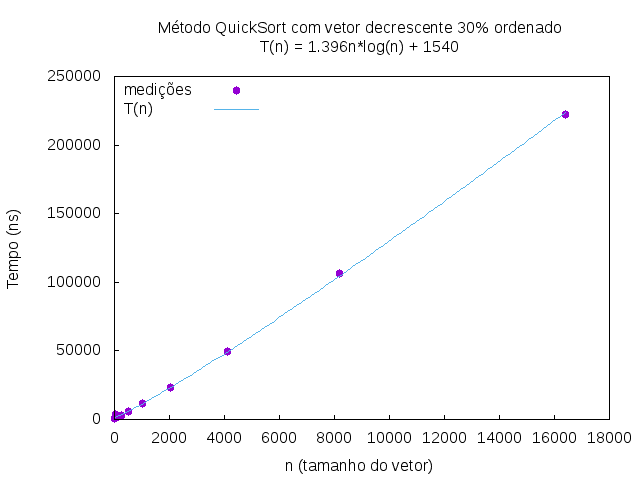
\includegraphics[width=0.7\linewidth]{graficos/QuickSort/vIntDecrescenteP30/vIntDecrescenteP30.png}
  \caption{Gráfico Quick Sort - Vetor Decrescente P30}
\end{figure}

\section{Quick Sort - Vetor Decrescente P40}
Tabela gerada utilizando Quick Sort com vetores de tamanho n, sendo n = $(2^k)$, de k = 4..14 e inseridos em ordem decrescente estando 40\% ordenado.
\begin{table}[H]
\centering
\caption{Quick Sort com vetor ordenado em ordem decrescente estando 40\% ordenado}
\label{my-label}
\begin{tabular}{|l|l|}
\hline
\multicolumn{1}{|c|}{\textbf{Número de Elementos}} & \multicolumn{1}{c|}{\textbf{Tempo de execução em nanosegundos}} \\ \hline
16 & 677 \\ \hline
32 & 905 \\ \hline
64 & 1706 \\ \hline
128 & 2646 \\ \hline
256 & 3768 \\ \hline
512 & 6826 \\ \hline
1024 & 12542 \\ \hline
2048 & 25469 \\ \hline
4096 & 62872 \\ \hline
8192 & 114528 \\ \hline
16384 & 229091 \\ \hline
\end{tabular}
\end{table}

\subsection{Gráfico Quick Sort - Vetor Decrescente P40}
\begin{figure}[H]
    \centering
    \includegraphics[width=0.7\linewidth]{graficos/QuickSort/vIntDecrescenteP40/vIntDecrescenteP40.png}
  \caption{Gráfico Quick Sort - Vetor Decrescente P40}
\end{figure}

\section{Quick Sort - Vetor Decrescente P50}
Tabela gerada utilizando Quick Sort com vetores de tamanho n, sendo n = $(2^k)$, de k = 4..14 e inseridos em ordem decrescente estando 50\% ordenado.
\begin{table}[H]
\centering
\caption{Quick Sort com vetor ordenado em ordem decrescente estando 50\% ordenado}
\label{my-label}
\begin{tabular}{|l|l|}
\hline
\multicolumn{1}{|c|}{\textbf{Número de Elementos}} & \multicolumn{1}{c|}{\textbf{Tempo de execução em nanosegundos}} \\ \hline
16 & 638 \\ \hline
32 & 803 \\ \hline
64 & 1209 \\ \hline
128 & 1954 \\ \hline
256 & 3424 \\ \hline
512 & 6323 \\ \hline
1024 & 12541 \\ \hline
2048 & 26206 \\ \hline
4096 & 54582 \\ \hline
8192 & 121376 \\ \hline
16384 & 239823 \\ \hline
\end{tabular}
\end{table}

\subsection{Gráfico Quick Sort - Vetor Decrescente P50}
\begin{figure}[H]
    \centering
    \includegraphics[width=0.7\linewidth]{graficos/QuickSort/vIntDecrescenteP50/vIntDecrescenteP50.png}
  \caption{Gráfico Quick Sort - Vetor Decrescente P50}
\end{figure}
\section{Observações Finais}
quick sort com vetor de elementos totalmente aleatório levaria aproximadamente 12 minutos para processar um vetor de $2^k$ com k = 32 elementos nessas condições.

\chapter{Counting Sort}
O algoritmo de ordenação Counting Sort é um algoritmo estável. Basicamente ele determina para cada entrada X, o número de elementos menor que ele, e utilizando essa informação, ele coloca o elemento x diretamente na posição correta no vetor de saída.
Em qualquer caso, temos que o algoritmo CountingSort tem complexidade de tempo O(n).

\section{Counting Sort - Vetor Aleatório}
Tabela gerada utilizando Counting Sort com vetores de tamanho n, sendo n = $(2^k)$, de k = 4..14 e inseridos aleatóriamente.
\begin{table}[H]
\centering
\caption{Counting Sort com vetor aleatório}
\label{my-label}
\begin{tabular}{|l|l|}
\hline
\multicolumn{1}{|c|}{\textbf{Número de Elementos}} & \multicolumn{1}{c|}{\textbf{Tempo de execução em nanosegundos}} \\ \hline
16 & 1180 \\ \hline
32 & 763 \\ \hline
64 & 753 \\ \hline
128 & 980 \\ \hline
256 & 1277 \\ \hline
512 & 3643 \\ \hline
1024 & 5315 \\ \hline
2048 & 12623 \\ \hline
4096 & 23526 \\ \hline
8192 & 64405 \\ \hline
16384 & 163553 \\ \hline
\end{tabular}
\end{table}

\subsection{Gráfico Counting Sort - Vetor Aleatório}
\begin{figure}[H]
    \centering
    \includegraphics[width=0.7\linewidth]{graficos/CountingSort/vIntAleatorio/vIntAleatorio.png}
  \caption{Gráfico Counting Sort - Vetor Aleatório}
\end{figure}

\section{Counting Sort - Vetor Crescente}
Tabela gerada utilizando Counting Sort com vetores de tamanho n, sendo n = $(2^k)$, de k = 4..14 e inseridos em ordem crescente.
\begin{table}[H]
\centering
\caption{Counting Sort com vetor ordenado em ordem crescente}
\label{my-label}
\begin{tabular}{|l|l|}
\hline
\multicolumn{1}{|c|}{\textbf{Número de Elementos}} & \multicolumn{1}{c|}{\textbf{Tempo de execução em nanosegundos}} \\ \hline
16 & 942 \\ \hline
32 & 665 \\ \hline
64 & 790 \\ \hline
128 & 1183 \\ \hline
256 & 1396 \\ \hline
512 & 2115 \\ \hline
1024 & 8305 \\ \hline
2048 & 17296 \\ \hline
4096 & 41228 \\ \hline
8192 & 59797 \\ \hline
16384 & 107430 \\ \hline
\end{tabular}
\end{table}

\subsection{Gráfico Counting Sort - Vetor Crescente}
\begin{figure}[H]
    \centering
    \includegraphics[width=0.7\linewidth]{graficos/CountingSort/vIntCrescente/vIntCrescente.png}
  \caption{Gráfico Counting Sort - Vetor Crescente}
\end{figure}

\section{Counting Sort - Vetor Crescente P10}
Tabela gerada utilizando Counting Sort com vetores de tamanho n, sendo n = $(2^k)$, de k = 4..14 e inseridos em ordem crescente estando 10\% ordenado.
\begin{table}[H]
\centering
\caption{Counting Sort com vetor ordenado em ordem crescente estando 10\% ordenado}
\label{my-label}
\begin{tabular}{|l|l|}
\hline
\multicolumn{1}{|c|}{\textbf{Número de Elementos}} & \multicolumn{1}{c|}{\textbf{Tempo de execução em nanosegundos}} \\ \hline
16 & 986 \\ \hline
32 & 703 \\ \hline
64 & 935 \\ \hline
128 & 1027 \\ \hline
256 & 1433 \\ \hline
512 & 2054 \\ \hline
1024 & 5931 \\ \hline
2048 & 16341 \\ \hline
4096 & 31788 \\ \hline
8192 & 73657 \\ \hline
16384 & 151634 \\ \hline
\end{tabular}
\end{table}

\subsection{Gráfico Counting Sort - Vetor Crescente P10}
\begin{figure}[H]
    \centering
    \includegraphics[width=0.7\linewidth]{graficos/CountingSort/vIntCrescenteP10/vIntCrescenteP10.png}
  \caption{Gráfico Counting Sort - Vetor Crescente P10}
\end{figure}

\section{Counting Sort - Vetor Crescente P20}
Tabela gerada utilizando Counting Sort com vetores de tamanho n, sendo n = $(2^k)$, de k = 4..14 e inseridos em ordem crescente estando 20\% ordenado.
\begin{table}[H]
\centering
\caption{Counting Sort com vetor ordenado em ordem crescente estando 20\% ordenado}
\label{my-label}
\begin{tabular}{|l|l|}
\hline
\multicolumn{1}{|c|}{\textbf{Número de Elementos}} & \multicolumn{1}{c|}{\textbf{Tempo de execução em nanosegundos}} \\ \hline
16 & 931 \\ \hline
32 & 698 \\ \hline
64 & 739 \\ \hline
128 & 983 \\ \hline
256 & 1409 \\ \hline
512 & 4075 \\ \hline
1024 & 5644 \\ \hline
2048 & 17222 \\ \hline
4096 & 28122 \\ \hline
8192 & 66564 \\ \hline
16384 & 102014 \\ \hline
\end{tabular}
\end{table}

\subsection{Gráfico Counting Sort - Vetor Crescente P20}
\begin{figure}[H]
    \centering
    \includegraphics[width=0.7\linewidth]{graficos/CountingSort/vIntCrescenteP20/vIntCrescenteP20.png}
  \caption{Gráfico Counting Sort - Vetor Crescente P20}
\end{figure}

\section{Counting Sort - Vetor Crescente P30}
Tabela gerada utilizando Counting Sort com vetores de tamanho n, sendo n = $(2^k)$, de k = 4..14 e inseridos em ordem crescente estando 30\% ordenado.
\begin{table}[H]
\centering
\caption{Counting Sort com vetor ordenado em ordem crescente estando 30\% ordenado}
\label{my-label}
\begin{tabular}{|l|l|}
\hline
\multicolumn{1}{|c|}{\textbf{Número de Elementos}} & \multicolumn{1}{c|}{\textbf{Tempo de execução em nanosegundos}} \\ \hline
16 & 884 \\ \hline
32 & 607 \\ \hline
64 & 793 \\ \hline
128 & 4111 \\ \hline
256 & 1340 \\ \hline
512 & 3869 \\ \hline
1024 & 6533 \\ \hline
2048 & 14310 \\ \hline
4096 & 33867 \\ \hline
8192 & 56900 \\ \hline
16384 & 117884 \\ \hline
\end{tabular}
\end{table}

\subsection{Gráfico Counting Sort - Vetor Crescente P30}
\begin{figure}[H]
    \centering
    \includegraphics[width=0.7\linewidth]{graficos/CountingSort/vIntCrescenteP30/vIntCrescenteP30.png}
  \caption{Gráfico Counting Sort - Vetor Crescente P30}
\end{figure}

\section{Counting Sort - Vetor Crescente P40}
Tabela gerada utilizando Counting Sort com vetores de tamanho n, sendo n = $(2^k)$, de k = 4..14 e inseridos em ordem crescente estando 40\% ordenado.
\begin{table}[H]
\centering
\caption{Counting Sort com vetor ordenado em ordem crescente estando 40\% ordenado}
\label{my-label}
\begin{tabular}{|l|l|}
\hline
\multicolumn{1}{|c|}{\textbf{Número de Elementos}} & \multicolumn{1}{c|}{\textbf{Tempo de execução em nanosegundos}} \\ \hline
16 & 1114 \\ \hline
32 & 644 \\ \hline
64 & 764 \\ \hline
128 & 1036 \\ \hline
256 & 1327 \\ \hline
512 & 1919 \\ \hline
1024 & 10465 \\ \hline
2048 & 18442 \\ \hline
4096 & 51975 \\ \hline
8192 & 56684 \\ \hline
16384 & 105513 \\ \hline
\end{tabular}
\end{table}

\subsection{Gráfico Counting Sort - Vetor Crescente P40}
\begin{figure}[H]
    \centering
    \includegraphics[width=0.7\linewidth]{graficos/CountingSort/vIntCrescenteP40/vIntCrescenteP40.png}
  \caption{Gráfico Counting Sort - Vetor Crescente P40}
\end{figure}

\section{Counting Sort - Vetor Crescente P50}
Tabela gerada utilizando Counting Sort com vetores de tamanho n, sendo n = $(2^k)$, de k = 4..14 e inseridos em ordem crescente estando 50\% ordenado.
\begin{table}[H]
\centering
\caption{Counting Sort com vetor ordenado em ordem crescente estando 50\% ordenado}
\label{my-label}
\begin{tabular}{|l|l|}
\hline
\multicolumn{1}{|c|}{\textbf{Número de Elementos}} & \multicolumn{1}{c|}{\textbf{Tempo de execução em nanosegundos}} \\ \hline
16 & 3878 \\ \hline
32 & 655 \\ \hline
64 & 771 \\ \hline
128 & 1086 \\ \hline
256 & 1391 \\ \hline
512 & 4088 \\ \hline
1024 & 5410 \\ \hline
2048 & 15451 \\ \hline
4096 & 29168 \\ \hline
8192 & 51542 \\ \hline
16384 & 114574 \\ \hline
\end{tabular}
\end{table}

\subsection{Gráfico Counting Sort - Vetor Crescente P50}
\begin{figure}[H]
    \centering
    \includegraphics[width=0.7\linewidth]{graficos/CountingSort/vIntCrescenteP50/vIntCrescenteP50.png}
  \caption{Gráfico Counting Sort - Vetor Crescente P50}
\end{figure}

\section{Counting Sort - Vetor Decrescente}
Tabela gerada utilizando Counting Sort com vetores de tamanho n, sendo n = $(2^k)$, de k = 4..14 e inseridos em ordem decrescente.
\begin{table}[H]
\centering
\caption{Counting Sort com vetor ordenado em ordem decrescente}
\label{my-label}
\begin{tabular}{|l|l|}
\hline
\multicolumn{1}{|c|}{\textbf{Número de Elementos}} & \multicolumn{1}{c|}{\textbf{Tempo de execução em nanosegundos}} \\ \hline
16 & 1111 \\ \hline
32 & 669 \\ \hline
64 & 807 \\ \hline
128 & 1038 \\ \hline
256 & 1308 \\ \hline
512 & 7100 \\ \hline
1024 & 5235 \\ \hline
2048 & 13556 \\ \hline
4096 & 31042 \\ \hline
8192 & 55271 \\ \hline
16384 & 121497 \\ \hline
\end{tabular}
\end{table}

\subsection{Gráfico Counting Sort - Vetor Decrescente}
\begin{figure}[H]
    \centering
    \includegraphics[width=0.7\linewidth]{graficos/CountingSort/vIntDecrescente/vIntDecrescente.png}
  \caption{Gráfico Counting Sort - Vetor Decrescente}
\end{figure}

\section{Counting Sort - Vetor Decrescente P10}
Tabela gerada utilizando Counting Sort com vetores de tamanho n, sendo n = $(2^k)$, de k = 4..14 e inseridos em ordem decrescente estando 10\% ordenado.
\begin{table}[H]
\centering
\caption{Counting Sort com vetor ordenado em ordem decrescente estando 10\% ordenado}
\label{my-label}
\begin{tabular}{|l|l|}
\hline
\multicolumn{1}{|c|}{\textbf{Número de Elementos}} & \multicolumn{1}{c|}{\textbf{Tempo de execução em nanosegundos}} \\ \hline
16 & 1035 \\ \hline
32 & 609 \\ \hline
64 & 784 \\ \hline
128 & 1082 \\ \hline
256 & 1326 \\ \hline
512 & 2019 \\ \hline
1024 & 5279 \\ \hline
2048 & 12392 \\ \hline
4096 & 25377 \\ \hline
8192 & 46191 \\ \hline
16384 & 93057 \\ \hline
\end{tabular}
\end{table}

\subsection{Gráfico Counting Sort - Vetor Decrescente P10}
\begin{figure}[H]
    \centering
    \includegraphics[width=0.7\linewidth]{graficos/CountingSort/vIntDecrescenteP10/vIntDecrescenteP10.png}
  \caption{Gráfico Counting Sort - Vetor Decrescente P10}
\end{figure}

\section{Counting Sort - Vetor Decrescente P20}
Tabela gerada utilizando Counting Sort com vetores de tamanho n, sendo n = $(2^k)$, de k = 4..14 e inseridos em ordem decrescente estando 20\% ordenado.
\begin{table}[H]
\centering
\caption{Counting Sort com vetor ordenado em ordem decrescente estando 20\% ordenado}
\label{my-label}
\begin{tabular}{|l|l|}
\hline
\multicolumn{1}{|c|}{\textbf{Número de Elementos}} & \multicolumn{1}{c|}{\textbf{Tempo de execução em nanosegundos}} \\ \hline
16 & 1251 \\ \hline
32 & 1486 \\ \hline
64 & 764 \\ \hline
128 & 1023 \\ \hline
256 & 1311 \\ \hline
512 & 3741 \\ \hline
1024 & 5552 \\ \hline
2048 & 13647 \\ \hline
4096 & 39382 \\ \hline
8192 & 48979 \\ \hline
16384 & 99118 \\ \hline
\end{tabular}
\end{table}

\subsection{Gráfico Counting Sort - Vetor Decrescente P20}
\begin{figure}[H]
    \centering
    \includegraphics[width=0.7\linewidth]{graficos/CountingSort/vIntDecrescenteP20/vIntDecrescenteP20.png}
  \caption{Gráfico Counting Sort - Vetor Decrescente P20}
\end{figure}

\section{Counting Sort - Vetor Decrescente P30}
Tabela gerada utilizando Counting Sort com vetores de tamanho n, sendo n = $(2^k)$, de k = 4..14 e inseridos em ordem decrescente estando 30\% ordenado.
\begin{table}[H]
\centering
\caption{Counting Sort com vetor ordenado em ordem decrescente estando 30\% ordenado}
\label{my-label}
\begin{tabular}{|l|l|}
\hline
\multicolumn{1}{|c|}{\textbf{Número de Elementos}} & \multicolumn{1}{c|}{\textbf{Tempo de execução em nanosegundos}} \\ \hline
16 & 1014 \\ \hline
32 & 676 \\ \hline
64 & 756 \\ \hline
128 & 1140 \\ \hline
256 & 1462 \\ \hline
512 & 4058 \\ \hline
1024 & 5755 \\ \hline
2048 & 16655 \\ \hline
4096 & 35422 \\ \hline
8192 & 64506 \\ \hline
16384 & 103663 \\ \hline
\end{tabular}
\end{table}

\subsection{Gráfico Counting Sort - Vetor Decrescente P30}
\begin{figure}[H]
    \centering
    \includegraphics[width=0.7\linewidth]{graficos/CountingSort/vIntDecrescenteP30/vIntDecrescenteP30.png}
  \caption{Gráfico Counting Sort - Vetor Decrescente P30}
\end{figure}

\section{Counting Sort - Vetor Decrescente P40}
Tabela gerada utilizando Counting Sort com vetores de tamanho n, sendo n = $(2^k)$, de k = 4..14 e inseridos em ordem decrescente estando 40\% ordenado.
\begin{table}[H]
\centering
\caption{Counting Sort com vetor ordenado em ordem decrescente estando 40\% ordenado}
\label{my-label}
\begin{tabular}{|l|l|}
\hline
\multicolumn{1}{|c|}{\textbf{Número de Elementos}} & \multicolumn{1}{c|}{\textbf{Tempo de execução em nanosegundos}} \\ \hline
16 & 1129 \\ \hline
32 & 705 \\ \hline
64 & 754 \\ \hline
128 & 1004 \\ \hline
256 & 1518 \\ \hline
512 & 1925 \\ \hline
1024 & 5353 \\ \hline
2048 & 12747 \\ \hline
4096 & 24478 \\ \hline
8192 & 49552 \\ \hline
16384 & 120622 \\ \hline
\end{tabular}
\end{table}

\subsection{Gráfico Counting Sort - Vetor Decrescente P40}
\begin{figure}[H]
    \centering
    \includegraphics[width=0.7\linewidth]{graficos/CountingSort/vIntDecrescenteP40/vIntDecrescenteP40.png}
  \caption{Gráfico Counting Sort - Vetor Decrescente P40}
\end{figure}

\section{Counting Sort - Vetor Decrescente P50}
Tabela gerada utilizando Counting Sort com vetores de tamanho n, sendo n = $(2^k)$, de k = 4..14 e inseridos em ordem decrescente estando 50\% ordenado.
\begin{table}[H]
\centering
\caption{Counting Sort com vetor ordenado em ordem decrescente estando 50\% ordenado}
\label{my-label}
\begin{tabular}{|l|l|}
\hline
\multicolumn{1}{|c|}{\textbf{Número de Elementos}} & \multicolumn{1}{c|}{\textbf{Tempo de execução em nanosegundos}} \\ \hline
16 & 960 \\ \hline
32 & 586 \\ \hline
64 & 792 \\ \hline
128 & 1090 \\ \hline
256 & 1344 \\ \hline
512 & 2043 \\ \hline
1024 & 5051 \\ \hline
2048 & 14108 \\ \hline
4096 & 26611 \\ \hline
8192 & 50560 \\ \hline
16384 & 140356 \\ \hline
\end{tabular}
\end{table}

\subsection{Gráfico Counting Sort - Vetor Decrescente P50}
\begin{figure}[H]
    \centering
    \includegraphics[width=0.7\linewidth]{graficos/CountingSort/vIntDecrescenteP50/vIntDecrescenteP50.png}
  \caption{Gráfico Counting Sort - Vetor Decrescente P50}
\end{figure}
\section{Observações Finais}
couting sort com vetor de elementos totalmente aleatório levaria aproximadamente 49 segundos para processar um vetor de $2^k$ com k = 32 elementos nessas condições.

\chapter{Radix Sort}
O algoritmo de ordenação Radix Sort é um algoritmo estável. Ele ordena itens que são identificados por chaves únicas. Cada chave é uma cadeia de caracteres ou número, o radix ordena as chaves. Ele ordena inteiros processando digitos indivíduais.
Em qualquer caso, temos que o algoritmo RadixSort tem complexidade de tempo O(n).

\section{Radix Sort - Vetor Aleatório}
Tabela gerada utilizando Radix Sort com vetores de tamanho n, sendo n = $(2^k)$, de k = 4..14 e inseridos aleatóriamente.
\begin{table}[H]
\centering
\caption{Radix Sort com vetor aleatório}
\label{my-label}
\begin{tabular}{|l|l|}
\hline
\multicolumn{1}{|c|}{\textbf{Número de Elementos}} & \multicolumn{1}{c|}{\textbf{Tempo de execução em nanosegundos}} \\ \hline
16 & 1773 \\ \hline
32 & 1345 \\ \hline
64 & 2116 \\ \hline
128 & 4744 \\ \hline
256 & 10074 \\ \hline
512 & 19320 \\ \hline
1024 & 50121 \\ \hline
2048 & 101591 \\ \hline
4096 & 224802 \\ \hline
8192 & 478058 \\ \hline
16384 & 1253961 \\ \hline
\end{tabular}
\end{table}

\subsection{Gráfico Radix Sort - Vetor Aleatório}
\begin{figure}[H]
    \centering
    \includegraphics[width=0.7\linewidth]{graficos/RadixSort/vIntAleatorio/vIntAleatorio.png}
  \caption{Gráfico Radix Sort - Vetor Aleatório}
\end{figure}

\section{Radix Sort - Vetor Crescente}
Tabela gerada utilizando Radix Sort com vetores de tamanho n, sendo n = $(2^k)$, de k = 4..14 e inseridos em ordem crescente.
\begin{table}[H]
\centering
\caption{Radix Sort com vetor ordenado em ordem crescente}
\label{my-label}
\begin{tabular}{|l|l|}
\hline
\multicolumn{1}{|c|}{\textbf{Número de Elementos}} & \multicolumn{1}{c|}{\textbf{Tempo de execução em nanosegundos}} \\ \hline
16 & 1257 \\ \hline
32 & 1550 \\ \hline
64 & 2657 \\ \hline
128 & 4851 \\ \hline
256 & 9156 \\ \hline
512 & 18680 \\ \hline
1024 & 51585 \\ \hline
2048 & 105519 \\ \hline
4096 & 208193 \\ \hline
8192 & 414850 \\ \hline
16384 & 1078854 \\ \hline
\end{tabular}
\end{table}

\subsection{Gráfico Radix Sort - Vetor Crescente}
\begin{figure}[H]
    \centering
    \includegraphics[width=0.7\linewidth]{graficos/RadixSort/vIntCrescente/vIntCrescente.png}
  \caption{Gráfico Radix Sort - Vetor Crescente}
\end{figure}

\section{Radix Sort - Vetor Crescente P10}
Tabela gerada utilizando Radix Sort com vetores de tamanho n, sendo n = $(2^k)$, de k = 4..14 e inseridos em ordem crescente estando 10\% ordenado.
\begin{table}[H]
\centering
\caption{Radix Sort com vetor ordenado em ordem crescente estando 10\% ordenado}
\label{my-label}
\begin{tabular}{|l|l|}
\hline
\multicolumn{1}{|c|}{\textbf{Número de Elementos}} & \multicolumn{1}{c|}{\textbf{Tempo de execução em nanosegundos}} \\ \hline
16 & 1449 \\ \hline
32 & 1470 \\ \hline
64 & 2184 \\ \hline
128 & 4827 \\ \hline
256 & 8697 \\ \hline
512 & 19543 \\ \hline
1024 & 58018 \\ \hline
2048 & 114081 \\ \hline
4096 & 266876 \\ \hline
8192 & 558293 \\ \hline
16384 & 1079561 \\ \hline
\end{tabular}
\end{table}

\subsection{Gráfico Radix Sort - Vetor Crescente P10}
\begin{figure}[H]
    \centering
    \includegraphics[width=0.7\linewidth]{graficos/RadixSort/vIntCrescenteP10/vIntCrescenteP10.png}
  \caption{Gráfico Radix Sort - Vetor Crescente P10}
\end{figure}

\section{Radix Sort - Vetor Crescente P20}
Tabela gerada utilizando Radix Sort com vetores de tamanho n, sendo n = $(2^k)$, de k = 4..14 e inseridos em ordem crescente estando 20\% ordenado.
\begin{table}[H]
\centering
\caption{Radix Sort com vetor ordenado em ordem crescente estando 20\% ordenado}
\label{my-label}
\begin{tabular}{|l|l|}
\hline
\multicolumn{1}{|c|}{\textbf{Número de Elementos}} & \multicolumn{1}{c|}{\textbf{Tempo de execução em nanosegundos}} \\ \hline
16 & 1569 \\ \hline
32 & 1443 \\ \hline
64 & 2196 \\ \hline
128 & 4695 \\ \hline
256 & 8532 \\ \hline
512 & 20225 \\ \hline
1024 & 50143 \\ \hline
2048 & 108896 \\ \hline
4096 & 215786 \\ \hline
8192 & 434859 \\ \hline
16384 & 1083653 \\ \hline
\end{tabular}
\end{table}

\subsection{Gráfico Radix Sort - Vetor Crescente P20}
\begin{figure}[H]
    \centering
    \includegraphics[width=0.7\linewidth]{graficos/RadixSort/vIntCrescenteP20/vIntCrescenteP20.png}
  \caption{Gráfico Radix Sort - Vetor Crescente P20}
\end{figure}

\section{Radix Sort - Vetor Crescente P30}
Tabela gerada utilizando Radix Sort com vetores de tamanho n, sendo n = $(2^k)$, de k = 4..14 e inseridos em ordem crescente estando 30\% ordenado.
\begin{table}[H]
\centering
\caption{Radix Sort com vetor ordenado em ordem crescente estando 30\% ordenado}
\label{my-label}
\begin{tabular}{|l|l|}
\hline
\multicolumn{1}{|c|}{\textbf{Número de Elementos}} & \multicolumn{1}{c|}{\textbf{Tempo de execução em nanosegundos}} \\ \hline
16 & 1566 \\ \hline
32 & 1507 \\ \hline
64 & 2394 \\ \hline
128 & 8107 \\ \hline
256 & 10217 \\ \hline
512 & 20026 \\ \hline
1024 & 52093 \\ \hline
2048 & 125015 \\ \hline
4096 & 315646 \\ \hline
8192 & 414589 \\ \hline
16384 & 1056987 \\ \hline
\end{tabular}
\end{table}

\subsection{Gráfico Radix Sort - Vetor Crescente P30}
\begin{figure}[H]
    \centering
    \includegraphics[width=0.7\linewidth]{graficos/RadixSort/vIntCrescenteP30/vIntCrescenteP30.png}
  \caption{Gráfico Radix Sort - Vetor Crescente P30}
\end{figure}

\section{Radix Sort - Vetor Crescente P40}
Tabela gerada utilizando Radix Sort com vetores de tamanho n, sendo n = $(2^k)$, de k = 4..14 e inseridos em ordem crescente estando 40\% ordenado.
\begin{table}[H]
\centering
\caption{Radix Sort com vetor ordenado em ordem crescente estando 40\% ordenado}
\label{my-label}
\begin{tabular}{|l|l|}
\hline
\multicolumn{1}{|c|}{\textbf{Número de Elementos}} & \multicolumn{1}{c|}{\textbf{Tempo de execução em nanosegundos}} \\ \hline
16 & 1511 \\ \hline
32 & 1449 \\ \hline
64 & 2159 \\ \hline
128 & 4897 \\ \hline
256 & 10195 \\ \hline
512 & 19773 \\ \hline
1024 & 50826 \\ \hline
2048 & 105839 \\ \hline
4096 & 228973 \\ \hline
8192 & 412796 \\ \hline
16384 & 1213010 \\ \hline
\end{tabular}
\end{table}

\subsection{Gráfico Radix Sort - Vetor Crescente P40}
\begin{figure}[H]
    \centering
    \includegraphics[width=0.7\linewidth]{graficos/RadixSort/vIntCrescenteP40/vIntCrescenteP40.png}
  \caption{Gráfico Radix Sort - Vetor Crescente P40}
\end{figure}

\section{Radix Sort - Vetor Crescente P50}
Tabela gerada utilizando Radix Sort com vetores de tamanho n, sendo n = $(2^k)$, de k = 4..14 e inseridos em ordem crescente estando 50\% ordenado.
\begin{table}[H]
\centering
\caption{Radix Sort com vetor ordenado em ordem crescente estando 50\% ordenado}
\label{my-label}
\begin{tabular}{|l|l|}
\hline
\multicolumn{1}{|c|}{\textbf{Número de Elementos}} & \multicolumn{1}{c|}{\textbf{Tempo de execução em nanosegundos}} \\ \hline
16 & 2771 \\ \hline
32 & 1584 \\ \hline
64 & 2927 \\ \hline
128 & 6718 \\ \hline
256 & 14551 \\ \hline
512 & 28748 \\ \hline
1024 & 83909 \\ \hline
2048 & 134313 \\ \hline
4096 & 205712 \\ \hline
8192 & 440127 \\ \hline
16384 & 1104181 \\ \hline
\end{tabular}
\end{table}

\subsection{Gráfico Radix Sort - Vetor Crescente P50}
\begin{figure}[H]
    \centering
    \includegraphics[width=0.7\linewidth]{graficos/RadixSort/vIntCrescenteP50/vIntCrescenteP50.png}
  \caption{Gráfico Radix Sort - Vetor Crescente P50}
\end{figure}

\section{Radix Sort - Vetor Decrescente}
Tabela gerada utilizando Radix Sort com vetores de tamanho n, sendo n = $(2^k)$, de k = 4..14 e inseridos em ordem decrescente.
\begin{table}[H]
\centering
\caption{Radix Sort com vetor ordenado em ordem decrescente}
\label{my-label}
\begin{tabular}{|l|l|}
\hline
\multicolumn{1}{|c|}{\textbf{Número de Elementos}} & \multicolumn{1}{c|}{\textbf{Tempo de execução em nanosegundos}} \\ \hline
16 & 1509 \\ \hline
32 & 1380 \\ \hline
64 & 2209 \\ \hline
128 & 4755 \\ \hline
256 & 10156 \\ \hline
512 & 21064 \\ \hline
1024 & 50785 \\ \hline
2048 & 105126 \\ \hline
4096 & 204012 \\ \hline
8192 & 421833 \\ \hline
16384 & 1300937 \\ \hline
\end{tabular}
\end{table}

\subsection{Gráfico Radix Sort - Vetor Decrescente}
\begin{figure}[H]
    \centering
    \includegraphics[width=0.7\linewidth]{graficos/RadixSort/vIntDecrescente/vIntDecrescente.png}
  \caption{Gráfico Radix Sort - Vetor Decrescente}
\end{figure}

\section{Radix Sort - Vetor Decrescente P10}
Tabela gerada utilizando Radix Sort com vetores de tamanho n, sendo n = $(2^k)$, de k = 4..14 e inseridos em ordem decrescente estando 10\% ordenado.
\begin{table}[H]
\centering
\caption{Radix Sort com vetor ordenado em ordem decrescente estando 10\% ordenado}
\label{my-label}
\begin{tabular}{|l|l|}
\hline
\multicolumn{1}{|c|}{\textbf{Número de Elementos}} & \multicolumn{1}{c|}{\textbf{Tempo de execução em nanosegundos}} \\ \hline
16 & 1575 \\ \hline
32 & 1407 \\ \hline
64 & 2223 \\ \hline
128 & 4714 \\ \hline
256 & 10106 \\ \hline
512 & 19246 \\ \hline
1024 & 49723 \\ \hline
2048 & 99033 \\ \hline
4096 & 196898 \\ \hline
8192 & 432726 \\ \hline
16384 & 1075879 \\ \hline
\end{tabular}
\end{table}

\subsection{Gráfico Radix Sort - Vetor Decrescente P10}
\begin{figure}[H]
    \centering
    \includegraphics[width=0.7\linewidth]{graficos/RadixSort/vIntDecrescenteP10/vIntDecrescenteP10.png}
  \caption{Gráfico Radix Sort - Vetor Decrescente P10}
\end{figure}

\section{Radix Sort - Vetor Decrescente P20}
Tabela gerada utilizando Radix Sort com vetores de tamanho n, sendo n = $(2^k)$, de k = 4..14 e inseridos em ordem decrescente estando 20\% ordenado.
\begin{table}[H]
\centering
\caption{Radix Sort com vetor ordenado em ordem decrescente estando 20\% ordenado}
\label{my-label}
\begin{tabular}{|l|l|}
\hline
\multicolumn{1}{|c|}{\textbf{Número de Elementos}} & \multicolumn{1}{c|}{\textbf{Tempo de execução em nanosegundos}} \\ \hline
16 & 1462 \\ \hline
32 & 1415 \\ \hline
64 & 2168 \\ \hline
128 & 4773 \\ \hline
256 & 12913 \\ \hline
512 & 18982 \\ \hline
1024 & 50323 \\ \hline
2048 & 102306 \\ \hline
4096 & 213200 \\ \hline
8192 & 425845 \\ \hline
16384 & 1280537 \\ \hline
\end{tabular}
\end{table}

\subsection{Gráfico Radix Sort - Vetor Decrescente P20}
\begin{figure}[H]
    \centering
    \includegraphics[width=0.7\linewidth]{graficos/RadixSort/vIntDecrescenteP20/vIntDecrescenteP20.png}
  \caption{Gráfico Radix Sort - Vetor Decrescente P20}
\end{figure}

\section{Radix Sort - Vetor Decrescente P30}
Tabela gerada utilizando Radix Sort com vetores de tamanho n, sendo n = $(2^k)$, de k = 4..14 e inseridos em ordem decrescente estando 30\% ordenado.
\begin{table}[H]
\centering
\caption{Radix Sort com vetor ordenado em ordem decrescente estando 30\% ordenado}
\label{my-label}
\begin{tabular}{|l|l|}
\hline
\multicolumn{1}{|c|}{\textbf{Número de Elementos}} & \multicolumn{1}{c|}{\textbf{Tempo de execução em nanosegundos}} \\ \hline
16 & 1642 \\ \hline
32 & 1432 \\ \hline
64 & 2173 \\ \hline
128 & 4948 \\ \hline
256 & 9691 \\ \hline
512 & 18212 \\ \hline
1024 & 49862 \\ \hline
2048 & 101564 \\ \hline
4096 & 206893 \\ \hline
8192 & 430726 \\ \hline
16384 & 1055471 \\ \hline
\end{tabular}
\end{table}

\subsection{Gráfico Radix Sort - Vetor Decrescente P30}
\begin{figure}[H]
    \centering
    \includegraphics[width=0.7\linewidth]{graficos/RadixSort/vIntDecrescenteP30/vIntDecrescenteP30.png}
  \caption{Gráfico Radix Sort - Vetor Decrescente P30}
\end{figure}

\section{Radix Sort - Vetor Decrescente P40}
Tabela gerada utilizando Radix Sort com vetores de tamanho n, sendo n = $(2^k)$, de k = 4..14 e inseridos em ordem decrescente estando 40\% ordenado.
\begin{table}[H]
\centering
\caption{Radix Sort com vetor ordenado em ordem decrescente estando 40\% ordenado}
\label{my-label}
\begin{tabular}{|l|l|}
\hline
\multicolumn{1}{|c|}{\textbf{Número de Elementos}} & \multicolumn{1}{c|}{\textbf{Tempo de execução em nanosegundos}} \\ \hline
16 & 1306 \\ \hline
32 & 1415 \\ \hline
64 & 2110 \\ \hline
128 & 5098 \\ \hline
256 & 9740 \\ \hline
512 & 19400 \\ \hline
1024 & 50306 \\ \hline
2048 & 107601 \\ \hline
4096 & 217893 \\ \hline
8192 & 469702 \\ \hline
16384 & 1141214 \\ \hline
\end{tabular}
\end{table}

\subsection{Gráfico Radix Sort - Vetor Decrescente P40}
\begin{figure}[H]
    \centering
    \includegraphics[width=0.7\linewidth]{graficos/RadixSort/vIntDecrescenteP40/vIntDecrescenteP40.png}
  \caption{Gráfico Radix Sort - Vetor Decrescente P40}
\end{figure}

\section{Radix Sort - Vetor Decrescente P50}
Tabela gerada utilizando Radix Sort com vetores de tamanho n, sendo n = $(2^k)$, de k = 4..14 e inseridos em ordem decrescente estando 50\% ordenado.
\begin{table}[H]
\centering
\caption{Radix Sort com vetor ordenado em ordem decrescente estando 50\% ordenado}
\label{my-label}
\begin{tabular}{|l|l|}
\hline
\multicolumn{1}{|c|}{\textbf{Número de Elementos}} & \multicolumn{1}{c|}{\textbf{Tempo de execução em nanosegundos}} \\ \hline
16 & 1511 \\ \hline
32 & 1456 \\ \hline
64 & 2208 \\ \hline
128 & 4801 \\ \hline
256 & 8646 \\ \hline
512 & 18827 \\ \hline
1024 & 50937 \\ \hline
2048 & 110078 \\ \hline
4096 & 226903 \\ \hline
8192 & 411363 \\ \hline
16384 & 1057336 \\ \hline
\end{tabular}
\end{table}

\subsection{Gráfico Radix Sort - Vetor Decrescente P50}
\begin{figure}[H]
    \centering
    \includegraphics[width=0.7\linewidth]{graficos/RadixSort/vIntDecrescenteP50/vIntDecrescenteP50.png}
  \caption{Gráfico Radix Sort - Vetor Decrescente P50}
\end{figure}
\section{Observações Finais}
hadix sort com vetor totalmente decrescente levaria aproximadamente 4 minutos e 34 segundos para processar um vetor de $2^k$ com k = 32 elementos.

\chapter{Bucket sort}
Bucket sort é um algoritmo de ordenação que funciona dividindo um vetor em um número finito de recipientes. Cada recipiente é então ordenado individualmente, seja usando um algoritmo de ordenação diferente, ou usando o algoritmo bucket sort recursivamente. Complexidade no pior caso O$(n^2)$ e no melhor caso caso O(n+k).
\section{Bucket sort - Vetor Aleatório}
Tabela gerada utilizando Bucket sort com vetores de tamanho n, sendo = $(2^k)$, k = 4...14 e inseridos aleatóriamente.
\begin{table}[H]
\centering
\caption{Bucket sort com Vetor aleatório}
\begin{tabular}{|l|l|}
\hline
\multicolumn{1}{|c|}{\textbf{Número de Elementos}} & \multicolumn{1}{c|}{\textbf{Tempo de execução em nanosegundos}} \\ \hline
16 & 1973 \\ \hline
32 & 1577 \\ \hline
64 & 3014 \\ \hline
128 & 8748 \\ \hline
256 & 23934 \\ \hline
512 & 89199 \\ \hline
1024 & 284571 \\ \hline
2048 & 1087923 \\ \hline
4096 & 4294051 \\ \hline
8192 & 16840640 \\ \hline
16384 & 66475936 \\ \hline
\end{tabular}
\end{table}


\subsection{Gráfico Bucket sort - Vetor Aletório}
\begin{figure}[H]
    \centering
    \includegraphics[width=0.7\linewidth]{graficos/Bucket/vIntAleatorio/vIntAleatorio.png}
  \caption{Gráfico Bucket sort - Vetor Aleatorio}
\end{figure}


\section{Bucket sort - Vetor Crescente}
Tabela gerada utilizando Bucket sort com vetores de tamanho n, sendo = $(2^k)$, k = 4...14 e inseridos em ordem crescente.

\begin{table}[H]
\centering
\caption{Bucket sort com Vetor ordenado em ordem crescente}
\label{my-label}
\begin{tabular}{|l|l|}
\hline
\multicolumn{1}{|c|}{\textbf{Número de Elementos}} & \multicolumn{1}{c|}{\textbf{Tempo de execução em nanosegundos}} \\ \hline
16 & 1462 \\ \hline
32 & 1276 \\ \hline
64 & 1598 \\ \hline
128 & 2201 \\ \hline
256 & 5808 \\ \hline
512 & 5298 \\ \hline
1024 & 8476 \\ \hline
2048 & 23017 \\ \hline
4096 & 57903 \\ \hline
8192 & 98423 \\ \hline
16384 & 218516 \\ \hline
\end{tabular}
\end{table}

\subsection{Grafico Bucket sort - Vetor Crescente}
\begin{figure}[H]
    \centering
    \includegraphics[width=0.7\linewidth]{graficos/Bucket/vIntCrescente/vIntCrescente.png}
  \caption{Gráfico Bucket sort - Vetor Crescente}
\end{figure}

\section{Bucket sort - Vetor Crescente P10}
Tabela gerada utilizando Bucket sort com vetores de tamanho n, sendo = $(2^k)$, k = 4...14 e inseridos em ordem crescente estando 10\% ordenado.

\begin{table}[H]
\centering
\caption{Bucket sort com Vetor ordenado em ordem crescente 10\% ordenado}
\label{my-label}
\begin{tabular}{|l|l|}
\hline
\multicolumn{1}{|c|}{\textbf{Número de Elementos}} & \multicolumn{1}{c|}{\textbf{Tempo de execução em nanosegundos}} \\ \hline
16 & 1225 \\ \hline
32 & 1321 \\ \hline
64 & 1898 \\ \hline
128 & 3800 \\ \hline
256 & 8864 \\ \hline
512 & 29263 \\ \hline
1024 & 112675 \\ \hline
2048 & 426087 \\ \hline
4096 & 1724471 \\ \hline
8192 & 6498292 \\ \hline
16384 & 25599240 \\ \hline
\end{tabular}
\end{table}

\subsection{Grafico Bucket sort - Vetor Crescente P10}
\begin{figure}[H]
    \centering
    \includegraphics[width=0.7\linewidth]{graficos/Bucket/vIntCrescenteP10/vIntCrescenteP10.png}
  \caption{Gráfico Bucket sort - Vetor Crescente P10}
\end{figure}

\section{Bucket sort - Vetor Crescente P20}
Tabela gerada utilizando Bucket sort com vetores de tamanho n, sendo = $(2^k)$, k = 4...14 e inseridos em ordem crescente estando 20\% ordenado.

\begin{table}[H]
\centering
\caption{Bucket sort com Vetor ordenado em ordem crescente 20\% ordenado}
\label{my-label}
\begin{tabular}{|l|l|}
\hline
\multicolumn{1}{|c|}{\textbf{Número de Elementos}} & \multicolumn{1}{c|}{\textbf{Tempo de execução em nanosegundos}} \\ \hline
16 & 1394 \\ \hline
32 & 1396 \\ \hline
64 & 2319 \\ \hline
128 & 5109 \\ \hline
256 & 14409 \\ \hline
512 & 54023 \\ \hline
1024 & 206030 \\ \hline
2048 & 782374 \\ \hline
4096 & 3106445 \\ \hline
8192 & 12244799 \\ \hline
16384 & 48165325 \\ \hline
\end{tabular}
\end{table}

\subsection{Grafico Bucket sort - Vetor Crescente P20}
\begin{figure}[H]
    \centering
    \includegraphics[width=0.7\linewidth]{graficos/Bucket/vIntCrescenteP20/vIntCrescenteP20.png}
  \caption{Gráfico Bucket sort - Vetor Crescente P20}
\end{figure}


\section{Bucket sort - Vetor Crescente P30}
Tabela gerada utilizando Bucket sort com vetores de tamanho n, sendo = $(2^k)$, k = 4...14 e inseridos em ordem crescente estando 30\% ordenado.

\begin{table}[H]
\centering
\caption{Bucket sort com Vetor ordenado em ordem crescente 30\% ordenado}
\label{my-label}
\begin{tabular}{|l|l|}
\hline
\multicolumn{1}{|c|}{\textbf{Número de Elementos}} & \multicolumn{1}{c|}{\textbf{Tempo de execução em nanosegundos}} \\ \hline
16 & 1420 \\ \hline
32 & 1477 \\ \hline
64 & 3137 \\ \hline
128 & 6966 \\ \hline
256 & 20704 \\ \hline
512 & 72550 \\ \hline
1024 & 276812 \\ \hline
2048 & 1088868 \\ \hline
4096 & 4363382 \\ \hline
8192 & 17125393 \\ \hline
16384 & 67952052 \\ \hline
\end{tabular}
\end{table}

\subsection{Grafico Bucket sort - Vetor Crescente P30}
\begin{figure}[H]
    \centering
    \includegraphics[width=0.7\linewidth]{graficos/Bucket/vIntCrescenteP30/vIntCrescenteP30.png}
  \caption{Gráfico Bucket sort - Vetor Crescente P30}
\end{figure}


\section{Bucket sort - Vetor Crescente P40}
Tabela gerada utilizando Bucket sort com vetores de tamanho n, sendo = $(2^k)$, k = 4...14 e inseridos em ordem crescente estando 40\% ordenado.

\begin{table}[H]
\centering
\caption{Bucket sort com Vetor ordenado em ordem crescente 40\% ordenado}
\label{my-label}
\begin{tabular}{|l|l|}
\hline
\multicolumn{1}{|c|}{\textbf{Número de Elementos}} & \multicolumn{1}{c|}{\textbf{Tempo de execução em nanosegundos}} \\ \hline
16 & 1535 \\ \hline
32 & 1722 \\ \hline
64 & 2884 \\ \hline
128 & 7462 \\ \hline
256 & 24820 \\ \hline
512 & 89196 \\ \hline
1024 & 346035 \\ \hline
2048 & 1363420 \\ \hline
4096 & 5462719 \\ \hline
8192 & 21522353 \\ \hline
16384 & 85206807 \\ \hline
\end{tabular}
\end{table}

\subsection{Grafico Bucket sort - Vetor Crescente P40}
\begin{figure}[H]
    \centering
    \includegraphics[width=0.7\linewidth]{graficos/Bucket/vIntCrescenteP40/vIntCrescenteP40.png}
  \caption{Gráfico Bucket sort - Vetor Crescente P40}
\end{figure}


\section{Bucket sort - Vetor Crescente P50}
Tabela gerada utilizando Bucket sort com vetores de tamanho n, sendo = $(2^k)$, k = 4...14 e inseridos em ordem crescente estando 50\% ordenado.

\begin{table}[H]
\centering
\caption{Bucket sort com Vetor ordenado em ordem crescente 50\% ordenado}
\label{my-label}
\begin{tabular}{|l|l|}
\hline
\multicolumn{1}{|c|}{\textbf{Número de Elementos}} & \multicolumn{1}{c|}{\textbf{Tempo de execução em nanosegundos}} \\ \hline
16 & 1495 \\ \hline
32 & 1722 \\ \hline
64 & 3257 \\ \hline
128 & 9138 \\ \hline
256 & 34405 \\ \hline
512 & 103202 \\ \hline
1024 & 427482 \\ \hline
2048 & 1597461 \\ \hline
4096 & 6416766 \\ \hline
8192 & 25148241 \\ \hline
16384 & 99797143 \\ \hline
\end{tabular}
\end{table}

\subsection{Grafico Bucket sort - Vetor Crescente P50}
\begin{figure}[H]
    \centering
    \includegraphics[width=0.7\linewidth]{graficos/Bucket/vIntCrescenteP50/vIntCrescenteP50.png}
  \caption{Gráfico Bucket sort - Vetor Crescente P50}
\end{figure}


\section{Bucket sort - Vetor Decrescente}
Tabela gerada utilizando Bucket sort com vetores de tamanho n, sendo = $(2^k)$, k = 4...14 e inseridos em ordem decrescente.

\begin{table}[H]
\centering
\caption{Bucket sort com Vetor ordenado em ordem decrescente}
\label{my-label}
\begin{tabular}{|l|l|}
\hline
\multicolumn{1}{|c|}{\textbf{Número de Elementos}} & \multicolumn{1}{c|}{\textbf{Tempo de execução em nanosegundos}} \\ \hline
16 & 1733 \\ \hline
32 & 1935 \\ \hline
64 & 3800 \\ \hline
128 & 10621 \\ \hline
256 & 35688 \\ \hline
512 & 134053 \\ \hline
1024 & 535638 \\ \hline
2048 & 2105018 \\ \hline
4096 & 8465724 \\ \hline
8192 & 33308407 \\ \hline
16384 & 132619442 \\ \hline
\end{tabular}
\end{table}

\subsection{Grafico Bucket sort - Vetor Decrescente}
\begin{figure}[H]
    \centering
    \includegraphics[width=0.7\linewidth]{graficos/Bucket/vIntDecrescente/vIntDecrescente.png}
  \caption{Gráfico Bucket sort - Vetor Decrescente}
\end{figure}


\section{Bucket sort - Vetor Decrescente P10}
Tabela gerada utilizando Bucket sort com vetores de tamanho n, sendo = $(2^k)$, k = 4...14 e inseridos em ordem descrescente estando 10\% ordenado.

\begin{table}[H]
\centering
\caption{Bucket sort com Vetor ordenado em ordem descrecente 10\% ordenado}
\label{my-label}
\begin{tabular}{|l|l|}
\hline
\multicolumn{1}{|c|}{\textbf{Número de Elementos}} & \multicolumn{1}{c|}{\textbf{Tempo de execução em nanosegundos}} \\ \hline
16 & 1652 \\ \hline
32 & 1926 \\ \hline
64 & 3661 \\ \hline
128 & 9606 \\ \hline
256 & 30709 \\ \hline
512 & 111680 \\ \hline
1024 & 444689 \\ \hline
2048 & 1735199 \\ \hline
4096 & 6904035 \\ \hline
8192 & 27147001 \\ \hline
16384 & 108381572 \\ \hline
\end{tabular}
\end{table}

\subsection{Grafico Bucket sort - Vetor Decrescente P10}
\begin{figure}[H]
    \centering
    \includegraphics[width=0.7\linewidth]{graficos/Bucket/vIntDecrescenteP10/vIntDecrescenteP10.png}
  \caption{Gráfico Bucket sort - Vetor Decrescente P10}
\end{figure}

\section{Bucket sort - Vetor Decrescente P20}
Tabela gerada utilizando Bucket sort com vetores de tamanho n, sendo = $(2^k)$, k = 4...14 e inseridos em ordem descrescente estando 20\% ordenado.

\begin{table}[H]
\centering
\caption{Bucket sort com Vetor ordenado em ordem descrecente 20\% ordenado}
\label{my-label}
\begin{tabular}{|l|l|}
\hline
\multicolumn{1}{|c|}{\textbf{Número de Elementos}} & \multicolumn{1}{c|}{\textbf{Tempo de execução em nanosegundos}} \\ \hline
16 & 1594 \\ \hline
32 & 1710 \\ \hline
64 & 3260 \\ \hline
128 & 8207 \\ \hline
256 & 25049 \\ \hline
512 & 89341 \\ \hline
1024 & 343952 \\ \hline
2048 & 1362340 \\ \hline
4096 & 5533807 \\ \hline
8192 & 21616313 \\ \hline
16384 & 86167002 \\ \hline
\end{tabular}
\end{table}

\subsection{Grafico Bucket sort - Vetor Decrescente P20}
\begin{figure}[H]
    \centering
    \includegraphics[width=0.7\linewidth]{graficos/Bucket/vIntDecrescenteP20/vIntDecrescenteP20.png}
  \caption{Gráfico Bucket sort - Vetor Decrescente P20}
\end{figure}

\section{Bucket sort - Vetor Decrescente P30}
Tabela gerada utilizando Bucket sort com vetores de tamanho n, sendo = $(2^k)$, k = 4...14 e inseridos em ordem descrescente estando 30\% ordenado.

\begin{table}[H]
\centering
\caption{Bucket sort com Vetor ordenado em ordem descrecente 30\% ordenado}
\label{my-label}
\begin{tabular}{|l|l|}
\hline
\multicolumn{1}{|c|}{\textbf{Número de Elementos}} & \multicolumn{1}{c|}{\textbf{Tempo de execução em nanosegundos}} \\ \hline
16 & 1615 \\ \hline
32 & 1701 \\ \hline
64 & 2935 \\ \hline
128 & 6735 \\ \hline
256 & 19846 \\ \hline
512 & 70981 \\ \hline
1024 & 267001 \\ \hline
2048 & 1048944 \\ \hline
4096 & 4196396 \\ \hline
8192 & 16480503 \\ \hline
16384 & 65337027 \\ \hline
\end{tabular}
\end{table}

\subsection{Grafico Bucket sort - Vetor Decrescente P30}
\begin{figure}[H]
    \centering
    \includegraphics[width=0.7\linewidth]{graficos/Bucket/vIntDecrescenteP30/vIntDecrescenteP30.png}
  \caption{Gráfico Bucket sort - Vetor Decrescente P30}
\end{figure}


\section{Bucket sort - Vetor Decrescente P40}
Tabela gerada utilizando Bucket sort com vetores de tamanho n, sendo = $(2^k)$, k = 4...14 e inseridos em ordem descrescente estando 40\% ordenado.

\begin{table}[H]
\centering
\caption{Bucket sort com Vetor ordenado em ordem descrecente 40\% ordenado}
\label{my-label}
\begin{tabular}{|l|l|}
\hline
\multicolumn{1}{|c|}{\textbf{Número de Elementos}} & \multicolumn{1}{c|}{\textbf{Tempo de execução em nanosegundos}} \\ \hline
16 & 1540 \\ \hline
32 & 1635 \\ \hline
64 & 2675 \\ \hline
128 & 5730 \\ \hline
256 & 15468 \\ \hline
512 & 53749 \\ \hline
1024 & 197174 \\ \hline
2048 & 783752 \\ \hline
4096 & 3138458 \\ \hline
8192 & 12246283 \\ \hline
16384 & 48159817 \\ \hline
\end{tabular}
\end{table}

\subsection{Grafico Bucket sort - Vetor Decrescente P40}
\begin{figure}[H]
    \centering
    \includegraphics[width=0.7\linewidth]{graficos/Bucket/vIntDecrescenteP40/vIntDecrescenteP40.png}
  \caption{Gráfico Bucket sort - Vetor Decrescente P40}
\end{figure}


\section{Bucket sort - Vetor Decrescente P50}
Tabela gerada utilizando Bucket sort com vetores de tamanho n, sendo = $(2^k)$, k = 4...14 e inseridos em ordem descrescente estando 50\% ordenado.

\begin{table}[H]
\centering
\caption{Bucket sort com Vetor ordenado em ordem descrecente 50\% ordenado}
\label{my-label}
\begin{tabular}{|l|l|}
\hline
\multicolumn{1}{|c|}{\textbf{Número de Elementos}} & \multicolumn{1}{c|}{\textbf{Tempo de execução em nanosegundos}} \\ \hline
16 & 1541 \\ \hline
32 & 1490 \\ \hline
64 & 2264 \\ \hline
128 & 4583 \\ \hline
256 & 11730 \\ \hline
512 & 38408 \\ \hline
1024 & 144989 \\ \hline
2048 & 539921 \\ \hline
4096 & 2153095 \\ \hline
8192 & 8579882 \\ \hline
16384 & 33392472s \\ \hline
\end{tabular}
\end{table}

\subsection{Grafico Bucket sort - Vetor Decrescente P50}
\begin{figure}[H]
    \centering
    \includegraphics[width=0.7\linewidth]{graficos/Bucket/vIntDecrescenteP50/vIntDecrescenteP50.png}
  \caption{Gráfico Bucket sort - Vetor Decrescente P50}
\end{figure}
\section{Observações Finais}
Bucket sort com vetor em ordem aleatória com $2^k$ com k = 32 elementos levaria aproximadamente 287 anos 2 meses e 30 dias para processar nessas condições.

%para ajuda
%\lstinputlisting[label={arq:prog1.c}, language=C, caption={Módulo Mínimo C}]{codigos/MiniC/prog1.c}
%\lstinputlisting[label={arq:prog4.c}, language=C, caption={Atribuição de uma soma de inteiros a uma variável C}]{codigos/MiniC/prog4.c}
%\begin{terminal}
%> sudo apt-get install llvm
%> sudo apt-get install clang
%\end{terminal}

\chapter{Referências}
\href{https://pt.wikipedia.org/wiki/Insertion_sort}{Insertion Sort}\\
\href{https://pt.wikipedia.org/wiki/Merge_sort}{Merge Sort}\\
\href{https://pt.wikipedia.org/wiki/Heapsort}{Heap Sort}\\
\href{https://en.wikipedia.org/wiki/Quicksort}{Quick Sort}\\
\href{https://pt.wikipedia.org/wiki/Counting_sort}{Counting Sort}\\
\href{https://en.wikipedia.org/wiki/Radix_sort}{Radix Sort}\\
\href{https://en.wikipedia.org/wiki/Bucket_sort}{Bucket Sort}\\
Introduction to algorithms 3rd Edition,Cormen, Thomas H,2009
  
\end{document} 
